%last minute:
%2 col
%check abstract


\def\conff{1}
%\def\conff{0}

\ifnum\conff=0
\documentclass[12pt]{article}
\fi

\ifnum\conff=1
\documentclass{sig-alternate-10pt}
\fi

\usepackage{times}
\usepackage{url}
\usepackage{comment}
\usepackage[english]{babel}
\usepackage{array}

%\usepackage{float}
%\floatstyle{ruled}
\usepackage{algorithm}
\usepackage{subfig}
\usepackage{amsmath}
\usepackage{amssymb}
\usepackage{wrapfig}
\usepackage{graphicx}
\graphicspath{{./Figs/}}

\usepackage{paralist}

\ifnum\conff=0
\usepackage[active]{srcltx}
\usepackage[a4paper]{geometry}
\geometry{hmargin=1in,top=1in}
\usepackage{setspace}%\singlespacing

\usepackage{amsthm}

\newtheorem{theorem}{Theorem}
\newtheorem{proposition}[theorem]{Proposition}
\newtheorem*{theoremnonum}{Theorem}
\newtheorem{lemma}[theorem]{Lemma}
\newtheorem{claim}[theorem]{Claim}
\newtheorem{coro}[theorem]{Corollary}
\newtheorem{remark}{Remark}
\newtheorem{observation}{observation}
\newtheorem{definition}{Definition}


\fi

%%%%%%%%%%%%%%%%%%%%%%%%%%%%%%%%%%%%%%%%%%%%%%%%%%%%%%%%%%%%%%%%%%%%%%%%%%%%%%%%%%%%%%%%%

% \newcommand{\qed}{$\blacksquare$}
% \newenvironment{proof}{\noindent {\bf Proof:} }{\hfill \qed}
\newenvironment{proof sketch}[1]{\noindent {\emph{Proof sketch of #1:}}}{\hfill \qed}

%%%%%%%%%%%%%%%%%%%%%%%%%%%%%%%%%%%%%%%%%%%%%%%%%%%%%%%%%%%%%%%%%%%%%%%%%%%%%%%%%%%%%%%%%


%\newenvironment{proof}{\noindent {\bfseries Proof.} }
%  {\mbox{}\nolinebreak \hfill \qed}
\newcommand{\eps}{\varepsilon}

\newcommand{\flow}{\text{\emph{flow}}}
\newcommand{\poly}{\text{\emph{poly}}}
\newcommand{\source}{\text{\emph{source}}}
\newcommand{\target}{\text{\emph{target}}}
\newcommand{\demand}{\text{\emph{demand}}}
\newcommand{\reject}{\text{\emph{reject}}}
%\newcommand{\load}{\text{\emph{load}}}
%\newcommand{\far}{R^{\text{\emph{Far}}}}
%\newcommand{\near}{R^{\text{\emph{Near}}}}
\newcommand{\opt}{\text{\textsc{opt}}}
\newcommand{\iopt}{I^*}
%\newcommand{\alg}{\textit{Alg}}
%\newcommand{\algf}{\textit{Alg}_{\text{\textit{far}}}}
%\newcommand{\algn}{\textit{Alg}_{\text{\textit{near}}}}
\newcommand{\eqdf}{\triangleq}

\newcommand{\SINR}{\text{\sc{sinr}}}
\newcommand{\SNR}{\text{\sc{snr}}}
\newcommand{\PER}{\text{\sc{per}}}
\newcommand{\pps}{\text{\emph{pps}}}
\newcommand{\hops}{\text{\emph{hops}}}
\newcommand{\mf}{\text{\emph{mf}}}
\newcommand{\MCS}{\text{\sc{mcs}}}
\newcommand{\Ein}{E_{\text{\emph{in}}}}
\newcommand{\Eout}{E_{\text{\emph{out}}}}
\newcommand{\RR}{\mathbb{R}}
\newcommand{\Imodel}{$\cal{I}$}

\newcommand{\algA}{\textsc{MF-I-S}}
\newcommand{\Alg}{\algA}
\newcommand{\algB}{\textsc{ShortP}}
\newcommand{\algC}{\textsc{MF-I}}
\newcommand{\algD}{\textsc{MF}}
\newcommand{\algE}{\textsc{MF-S}}

\newcommand{\algS}{\algB}

\begin{document}
%\begin{titlepage}
\title{Real-Time Video Streaming in Multi-hop Wireless Static Ad Hoc Networks}

\ifnum\conff=0
\author{%
Guy Even\thanks{School of Electrical Engineering,
Tel-Aviv Univ., Tel-Aviv 69978, Israel.
\protect\url{{guy,medinamo,moni,sasha}@eng.tau.ac.il}}
\and
Yaniv Fais$^*$
\and
Moti Medina$^*$
%
\and Shimon (Moni) Shahar$^*$
\and Alexander Zadorojniy$^*$ }
\fi
\date{}

\maketitle


%%% ----------------------------------------------------------------------

\begin{abstract}
  In this paper we deal with the problem of streaming multiple video
  streams between pairs of nodes in a multi-hop wireless ad hoc
  network.  The nodes are positioned on a plane, know their locations,
  and are synchronized (via GPS). We consider a 802.11g WiFi network
  in which NICs can hop between non-overlapping frequency channels in
  a synchronous fashion. Our goal is to maximize the minimum
  throughput over all the video streams. We designed a centralized
  algorithm that computes a channel/time-slot table.  Each entry in
  the table specifies the active links.

  Our algorithm constructs a communication graph based on distances.
  For each link in the communication graph, a set of interfering links
  is defined based on distances and the SNR of the link.  A
  multicommodity flow with interference constraints is solved by
  linear programming. The flow is then rounded to obtain the
  channel/time-slot table. After the table is broadcast, each node
  receives and transmits according to the table. In addition, we developed a localized
  flow-control mechanism to stabilize the queue lengths.

  We simulated our algorithm using OMNET++/MixiM (i.e., physical SINR
  interference model) to test whether the computed throughput is
  achieved. Our results show that we are able to route 70\% of the
  computed throughput.
\end{abstract}

\begin{comment}
  \paragraph{ Keywords:}
\end{comment}

%\end{titlepage}
\section{Introduction}

We address the problem of routing real-time video streams in static ad
hoc wireless networks.  Our goal is to develop and implement an
efficient algorithm and test it in the realistic physical model.

\paragraph{Special characteristics of real-time video streaming}
Streaming of real-time video in a multi-hop ad hoc network is a
challenging task.  We briefly overview these unique characteristics.
\begin{inparaenum}[(1)]
%  \item Video coding (e.g., H.264/MPEG) creates a bursty stream since
%    I-frames are much longer than the other frames. One could smoothen
%    the stream at the cost of incurring a extra delay of a second
%    (i.e., the time between I-frames).
\item End-to-end delay in streaming of real-time video should be as
  small as possible.  We assume that a delay of $1$-$2$ seconds is
  tolerable if the video has to travel across $10$ hops.  One
  implication of this constraint is that end-to-end acknowledgments and TCP are
  not an option.
\item Unless erasure codes are employed, loosing even a small fraction
  of the packets incurs an intolerable degradation in the video
  quality. We assume that video has acceptable quality if less that
  $0.5\%$ of the packets are dropped. In wireless networks, each link
  can have a \PER\ of $1\%$-$5\%$. Thus, after $10$ hops, one is left
  with intolerable erasures.  On the other had, erasure codes incur an
  extra end-to-end delay since they need to accumulate data for a
  block before encoding can take place. This means that relying on
  WiFi acknowledgments and retransmit capabilities can be useful to
  avoid packet drops if the \PER\ is small.
\item A useful feature in video coding is the ability to adjust the
  compressed bit-rate. This means that the video encoder can be
  continuously controlled to generate a video stream of a requested
  bit rate. We rely on this feature in our flow control algorithm.
  This feature separates video streaming from other applications such
  as FTP.
\end{inparaenum}
The necessity of cross layer designs has been recognized for
satisfying the special characteristics of real-time video streaming
over wireless
networks~\cite{shan2005cross,setton2005cross,khan2006application}.  We
continue this line of work.
\paragraph{Previous Work}

The WiFi technology builds on the 802.11 protocol, where in this paper
we used the 802.11g standard. The exact details of the communication,
such as RTS/CTS frames, and hold off time are described in detail in
~\cite{gast2005802}. The standard has 8 Modulation Coding Schemes
(\MCS) that define the data-rate, coding and modulation. The \MCS s
are ordered from a rate of 6Mbps for \MCS\ $0$ to rate of 54Mbps for
\MCS\ $7$.  The higher the data-rate, the higher the required
signal-to-noise ratio (\SNR). Adapting the \MCS\ is one of the ways to
decrease the error rate in case of change in the \SNR
~\cite{kamerman1997wavelan,holland2001rate}.

The multi-hop routing problem for ad hoc networks was investigated
thoroughly.  While our emphasis is on supporting video streams (i.e.,
throughout and low end-to-end delay), the main of research focuses on
distributed algorithms for packet routing in the case of mobile
nodes~\cite{johnson1996dynamic,broch1998performance,perkins2002ad}.

One of the commonly used heuristics for routing is based on finding
paths with maximum bottleneck, namely, paths for which the edge with
the lowest capacity is maximum ~\cite{draves2004routing}. In
~\cite{draves2004routing}, the goal function is a combination of
maximizing the bottleneck and the total throughput. We used this
algorithm in our benchmarks (we call it \algS). A different approach
for the routing problem is based on solving a linear program. In
~\cite{jain2005impact} Jain et al. used the graph based protocol
interference model to approximate the physical \SINR-interference
model. The protocol model is an approximation to the physical
\SINR-interference model, since interference from links may accumulate
and create an interference.  In~\cite{jain2005impact}, an linear
program (LP) is formulated for the problem of routing multiple
streams. The LP uses constraints that are based on independent sets in
a conflict graph. This method is not polynomial time.  Simulations
in~\cite{jain2005impact} were run with nodes on a grid, however, these
simulations are not in the physical model.
Following~\cite{jain2005impact}, Alicherry et al
~\cite{alicherry2005joint11} formulated a linear program that can be
computed in polynomial time.  They simulated their algorithm on a grid
and on random scenarios. A similar LP was formulated also in
~\cite{buragohain2007improved}. Wan~\cite{wan2009multiflows} pointed
out various errors in previous algorithms and presented a new linear
program that corrects the problem. He proved that: (i) there is a
$23$-approximation algorithm based on the linear program, and (ii)
there is a polynomial time scheme (PTAS) for the problem, however,
this PTAS is not practical. The linear program presented
in~\cite{wan2009multiflows} is more complicated than the LP
in~\cite{alicherry2005joint11,buragohain2007improved} and is harder to
solve. It is not clear if Wan's method is efficient enough to work
even with moderate sized networks.


\paragraph{Our Contributions}
\begin{enumerate}
\item To evaluate our algorithm we perform a simulation of real-time
  video streaming in a standard 802.11g setting using OMNET++/MixiM
  (Sec.~\ref{sec:exp}).  In this setting, all WiFi frames are
  transmitted (i.e., RTS,CTS, packet, ACK), and interferences between
  frames are analyzed using the SINR and the MCS.
\item We introduce a new interference model that is an intermediate
  model between the physical \SINR-model and the graph based protocol
  model (Sec.~\ref{sec:models}). The interference set of a link is a
  function of the signal-to-noise ratio of the link and the \MCS\ of
  the link.  As the link is closer to the \SINR-threshold, the
  interference set grows, so that \SINR\ is not in the ``waterfall''
  region of the \PER\ function.  One advantage of this new
  interference model is that it is easy to formulate interference
  constraints in the linear program formulation (Sec.~\ref{sec:LP}).
\item We formulate the problem of minimizing end-to-end delay due to a
  schedule that supports a given multi-flow. We developed and
  implemented a scheduler algorithm that address this problem of
  reducing end-to-end delays while supporting a similar throughput.
  (Sec~\ref{sec:sched}).
\item We developed and implemented a flow control algorithm that
  stabilizes the queue lengths and controls the data-rate along the
  links.  This flow control algorithm is executed locally by the
  nodes.
\item We combine the various aspects of video streaming to analyze
  performance that is crucial for real-time video streaming.  Namely,
  we measured the throughput, end-to-end delay, fraction of dropped
  packets, and the stability of these parameters.
\end{enumerate}
\begin{comment}
  
\paragraph{Techniques}
\textbf{KEEP?}  The algorithm computes two tables: a multi-flow table
$\mf$ and a time-slotted frequency table $A$ that governs
communication in the network. Each entry $A[j,t]$ of the table is
indexed by a frequency channel $j$ and a time slot $t$ pair.  The set
of links that appear in $A[j,t]$ are supposed to deliver packets in
time slot $t$ using the frequency channel $j$.


The algorithm computes a
\paragraph{Organization}
\end{comment}
\section{Problem Definition}\label{sec:problem}
\paragraph{Setting}
We consider a WiFi 802.11g static ad hoc network with $3$ non-interfering radio
channels with the assumptions:
\begin{inparaenum}[(i)]
\item Single radio: each node has a single wireless network interface
  controller (WNIC).
\item Each node is equipped with a GPS so that it knows
  its location and the nodes are synchronized.
\item The WNICs support quick synchronized hops between frequency
  channels.
\item Isotropic antennas.
\item We also assume that the nodes have already joined the network
  and that there is at least one node (i.e., center node) that holds
  full information about the network (i.e., nodes and locations).
  Accumulating this information can be done in a distributed
  low-bandwidth fashion after building a spanning
  tree~\cite{awerbuch1987optimal}.
\end{inparaenum}




\paragraph{Problem Definition}
The input to the algorithms consists of:
\begin{enumerate}
\item A set $V$ of $n$ nodes in the plane. A transceiver is located in
  each node.
\item A set of $k$ video stream requests $\{r_i\}_{i=1}^k$. Each
  stream request is a triple $r_i\eqdf (a_i,b_i,d^*_i)$, where $a_i$ is
  the source (e.g., camera) of the stream, $b_i$ is the destination,
  and $d^*_i$ is the required data-rate.
\end{enumerate}
Ideally, we would like to satisfy all the requests, namely, for each
video stream $r_i$, route packets using multi-hops from $a_i$ to $b_i$.
We assume that there is there is a path in the network between each
source-destination pair.

Let $d_i$ denote the data-rate achieved for the $i$th stream.  The
service ratio $\rho_i$ of the $i$th demand is defined by $\rho_i \eqdf
d_i/d^*_i$.  Our goal is to maximize the minimum service ratio,
namely, $\max \min_i \rho_i$.

Additional performance measures are:
\begin{inparaenum}[(i)]
\item End-to-end delay - this is the time it takes a packet to reach
  its destination. We are interested in reducing the maximum delay
  (among the packets that are delivered) since the video is real-time.
  In addition, the maximum delay determines the size of the jitter
  buffer in the receiving side.
\item Number of dropped packets. Queue management may drop packets
  that never reach their destination.
\item Queue lengths in intermediate nodes tell us how much memory
  should be allocated and also give an indication of the delay per hop.
\end{inparaenum}

\section{Preliminaries}
\label{sec:prelim}

\subsection{Interference Models}

\paragraph{Bidirectional interference}
The delivery of a message in the WiFi MAC requires transmission of
frames by both sides (e.g., RTS and packet are transmitted by the
sender, CTS and ACK are transmitted by the receiver). Hence,
interferences can be caused also by frames transmitted by a the
receiving side.

\noindent
We outline the three interference models below.
\paragraph{The SINR model}
The SINR model, also called the physical
interference model, defines successful communication as follows.  Let
$d_{u,v}$ denote the distance between nodes $u$ and $v$.  Suppose a subset
$S_t\subseteq V$ of the nodes are transmitting simultaneously in the
same frequency channel as $u$.  The signal-to-interference-plus-noise
ratio (SINR) for the reception by $v\in V\setminus S_t$ of the signal
transmitted by $u\in S_t$ in the presence of the transmitters $S_t$ is
defined by
\[
\SINR(u,v,S_t) \eqdf \frac{P/d_{u,v}^{\alpha}}{N+\sum_{x\in
    S_t\setminus{u}} P/d_{x,v}^{\alpha}}.
\]
Each transmitter can use one of several modulation coding schemes (\MCS).
The message transmitted by $u$ in an \MCS\ $m$ is successfully received by
$v$ if $\SINR(u,v,S_t)\geq \beta_m$, where $\beta_m$ is the minimum
SINR-threshold for the \MCS\ $m$.

\paragraph{Protocol model}
The protocol model, also called the graph model, is specified by two
radii:
\begin{inparaenum}[(i)]
\item A communication distance $r$.
\item An interference distance $R$.
\end{inparaenum}
The rule for successful communication between two nodes $u$ and $v$ is
that $v$ receives the message from $u$ if $d_{u,v}<r$ and every node
$x$ that transmits at the same time satisfies $d_{xv}> R$.  In this
model, a communication graph is defined over the nodes.  Two nodes are
linked by an edge if their distance is less than the communication
distance $r$.

Since the WiFi MAC requires transmission by both sides, an
\emph{interference} is defined between two links $(u,v)$ and $(u',v')$
if $\min\{d_{u,u'},d_{u,v'}, d_{v,u'}, d_{v,v'}\} < R$.  We say that a
subset $L$ of links is \emph{non-interfering} if no two links in $L$
interfere.  In the protocol model, a \emph{schedule} is a sequence
$\{L_i\}_i$ of subsets of non-interfering links.


\paragraph{The new model}
The new model is an intermediate model between the SINR model and the
protocol model. The idea is that, as the \SNR\ of a link grows, the
link can tolerate more interference. Hence, the interference distance
is not fixed.

Consider a pair $(u,v)$ of nodes and an \MCS\ $m$.
The triple $(u,v,m)$ is a \emph{link} in the new model if
$\SINR(u,v,\emptyset) \geq \beta_m$.

Since both sides of a link transmit and receive, the interference set
of a link must take into account interferences caused by other
transmissions both in the receiver and the sender. However, the frames
sent by the receiving side are in \MCS\ $0$, therefore, reception of
these frames depends on the $\SINR$-threshold $\beta_0$.

The interference set $V_{u,v,m}$ of the link $e=(u,v,m)$ is defined by
  \begin{align*}
    V_{u,v,m} \eqdf \left\{ x \in V \setminus\{u\}\right. &\left | \SINR(u,v,\{x\}) \geq \mu  \cdot \beta_i \text{ or } \right. \\
    & \left.\SINR(v,u,\{x\}) \geq \mu \cdot \beta_0\right\}.
\end{align*}
The motivation for this definition is that transmissions of nodes in $V_{u,v,m}$ interfere with
the reception of $v$ by $u$, or vice versa.
The choice of $\mu=1.585$ gives us a margin of $2$dB above the
\SINR-threshold.  This margin keeps the $\SINR$ above the threshold
due to interferences caused by transmitters not in $S_{u,v,m}$.

We also define the interfering set of edges with respect to the link $e=(u,v,m)$.
\begin{align*}
  I_{u,v,m} \eqdf \{ e'=(u',v',m') \mid &\{u',v'\} \cap (V_{u,v,m} \cup V_{v,u,m})
\\
& \neq \emptyset\} \setminus \{(u,v,m)\}.
\end{align*}
The interference set $I_{u,v,m}$ contains a link $e'$ if either
endpoint of $e'$ interferes with reception at the endpoints $u$ or
$v$.

\begin{comment}
  \begin{align*}
    S_{u,v,m} &\eqdf \left\{ x \in V \left | \frac{1}{6}\cdot
        \frac{P}{d_{x,v}^{\alpha}} > \left( \frac{P}{\beta\cdot
            d_{u,v}^{\alpha}} - N \right) \right.  \right\}
  \end{align*}
The justification for the definition of the interference set is summarized in the following claim.
\begin{claim}
Suppose $S_t$ is ``feasible''.
If $S_t \cap S_{u,v,m}=\emptyset$ then
$\SINR(u,v,S_t) \geq \SINR (u,v,\emptyset) \cdot \gamma.$
\end{claim}
\end{comment}

\subsection{Notation}

Let $u$ and $v$ denote nodes and $m$ denote an \MCS.  A link is a
triple $(u,v,m)$ such that $\SINR(u,v,\emptyset)\geq \beta_m$.  This
definition implies that there can be multiple parallel links between
$u$ and $v$, each with a different \MCS.

We denote the set of links by $E$. The set $\Eout(v)$ (resp.
$\Ein(v)$) denotes the set of links that emanate from (resp. enter)
$v$. Let $E(v)$ denote the set of links $\Ein(v)\cup \Eout(v)$.

For a link $e=(u,v,m)$, let $\MCS(e)=m$, i.e., the \MCS\ $m$ of the link $e$.



\section{Algorithm}\label{sec:outline}
\subsection{Networks Governed by Time-Slotted Frequency Tables}
Two tables govern the communication in the network.  The first table
$A$ is a time-slotted frequency table. The dimensions of $A$ are
$F\times T$, where $F$ denotes the number of frequency channels and
$T$ denotes the number of time slots.  There is one row for each
frequency channel and one column for each time slot. (In our
implementation we used $F=3$ and $T=200$).  The table $A$ determines a
periodic schedule.  The second table is a multi-flow table $\mf$. The
dimensions of $\mf$ are $|E|\times [1..k]$ (recall that $k$ equals the
number of video streams).  The entry $\mf(e,s)$ specifies the number
of packets-per-period that should be delivered along link $e$ for
stream $s$.

Each table entry $A[j,t]$ is a subset of links,
i.e., $A[j,t]\subseteq E$.  The table governs communication in the
sense that, in slot $t'$, the links in $A[j,t' \pmod T]$ try to deliver packets
using frequency channel $j$.

We use $A[\cdot,t]$ to denote the set of links $\cup_{j\in F}
A[j,t]$.  Since we assume that each node is equipped is a single
radio, it follows that two links that share an endpoint cannot be
active in the same time slot.  Hence, for every node $v$, $E(v) \cap
A[\cdot ,t]$ may contain at most one link.

Algorithm \Alg\ computes a time-slotted frequency table that supports
a multi-flow (see Sec.~\ref{sec:output}). A time-slotted frequency
tables schedules active links as listed in Algorithm~\ref{alg:tx-rx}.
Each node $v$ executes Algorithm TX-RX$(v)$ locally.  Since $E(v) \cap
A[\cdot ,t]$ may contain at most one link, a node $v$ is either a
receiver, a sender, or inactive in each time slot.  We elaborate below how
a queue $Q(v,s)$ with the highest priority for transmission along link
$e$ in line~\ref{line:priority} in the Transmit procedure is defined.

Upon invocation of Transmit$(e,j)$, where $e=(v,u,m)$, the node $v$
needs to decide which packet to transmit. The node $v$ uses the
multi-flow table $\mf$ to determine the set $S_e$ of streams that are
routed along $e$.  Since delay is a major issue, it is reasonable to
use an EDD-like policy, i.e., pick the oldest packet in the queues
$Q(v,s)$, for $s\in S_e$.  However, such a policy ignores the
remaining number of hops a packet needs to traverse. We prefer the
approach that emphasizes fairness. That is, assign a priority that
equals the ratio of the number of packets of stream $s$ transmitted
along $e$ in the last period divided by the required number. The lower
this ratio, the higher priority of the stream. This approach also
combines well with the flow control algorithm described in
Sec.~\ref{sec:flow control}.


\begin{algorithm}
  \caption{TX-RX$(v)$ - a local transmit-receive algorithm for node
    $v$ as specified by a time-slotted frequency table $A$.}
\label{alg:tx-rx}
For time slot $t'=0$ to $\infty$ do
  \begin{enumerate}%1
\item $t = t' \pmod T$.
  \item if $\Ein(v)\cap A[\cdot,t ]\neq \emptyset$ then
    \{reception mode\}
    \begin{enumerate}%2
    \item Let $e\in \Ein(v)\cap A[\cdot,t]$, where $e(u,v,m)\in
      A[j,t]$.
    \item While slot $t$ is not over call Receive$(e,j)$.
    \end{enumerate}%2
  \item if $\Eout(v)\cap A[\cdot,t ]\neq \emptyset$ then
    \{transmission mode\}
    \begin{enumerate}%2
    \item Let $e\in \Eout(v)\cap A[\cdot,t ]$, where
      $e(v,u,m)\in A[j,t]$.
    \item While slot $t$ is not over call Transmit$(e,j)$.
    \end{enumerate}%2
  \end{enumerate}%1
Receive$(e,j)$ - where link $e=(u,v,m)$ and $j$ is a frequency channel.
\begin{enumerate}
\item Set tuner to reception in frequency channel $j$.
\item Upon reception of a packet $p$ from stream $s$, insert $p$ to $Q(v,s)$.
\end{enumerate}

Transmit$(e,j)$-  where link $e=(v,u,m)$ and $j$ is a frequency channel.
\begin{enumerate}
\item Set tuner to transmission in frequency channel $j$.
\item\label{line:priority} Pick a queue $Q(v,s)$ with a highest priority for transmission along $e$.
\item $p \gets DEQUEUE(Q(v,s))$.
\item Transmit $p$ along $e$.
\end{enumerate}
\end{algorithm}

\subsection{Algorithm Specification}
\paragraph{Input}
The input to Algorithm \Alg\ consists of the following:
\begin{enumerate}
\item A set $V\subseteq \RR^2$  of nodes in the plane.
\item A set of $k$ video stream requests $\{r_i\}_{i=1}^k$. Each
  request $r_i$ is a triple $r_i\eqdf (a_i,b_i,d^*_i)$, where $a_i$ is
  the source (e.g., camera) of the stream, $b_i$ is the destination,
  and $d^*_i$ is the required data-rate.
\end{enumerate}
\paragraph{Output}
\label{sec:output}
The output of Algorithm \Alg\ consists of two parts:
\begin{inparaenum}[(i)]
\item a time-slotted frequency table $A$, and
\item a multi-flow $\mf(e,s)$, for every link $e$ and stream $1\leq
  s\leq k$.
\end{inparaenum}
We note that the units of flow are packets-per-period, where the
period is the duration of a time slot times the number $T$ of
time-slots in a period.

The multi-flow $\mf(e,s)$ determines the routing and the throughout of
each stream. The role of the frequency/time-slot table $A$ is to
specify a periodic schedule that determines which links are active in
which time slots.

Although we use fixed length packets (e.g., 2KB), the \MCS\ of a link
determines the amount of time required for completing the delivery of
a packet.  This means, that within one time slot, multiple packets may
be delivered along a single link.  Let $\pps(e)$ denote the number of
packets-per-slot that can be delivered along $e$.  Namely, node $u$
can transmit at most $\pps(e)$ packets to node $v$ along link
$e=(u,v,m)$ in one time-slot. Note that the value of $\pps(e)$ is a function of
the \MCS\ of the link $e$.

\medskip \noindent
The table $A$ should satisfy the following properties:
\begin{enumerate}
\item Every entry $A[j,t]$ in the table is a set of non-interfering
  links (in an interference model \Imodel). Thus the links in $A[j,t]$
  may be active simultaneously.
\item The data-rates $\mf(e,s)$ are supported by the table. Namely,
  \begin{align*}
    \sum_{s=1}^k \mf(e,s) \leq |\{A[j,t] \mid e\in A[j,t]\}|\cdot \pps(e),
  \end{align*}
\end{enumerate}

\subsection{Algorithm Description}
The algorithm consists of two parts: (i)~computation of a
multi-commodity flow with conflict constraints, and (ii)~scheduling of
the multi-commodity flow in a time-slotted frequency table.
We elaborate on each of these parts.

\paragraph{Multi-commodity flow with conflict constraints}
We formulate the problem of routing and scheduling the video streams
by a linear program (LP).  A similar LP is used
in~\cite{alicherry2005joint11,buragohain2007improved} with respect to
the protocol interference model.  We use our new interference model
for the interference constraints.

For each requested stream $r_i$, we define the supply ratio $\rho_i$
to be the ratio between the flow allocated to the $i$'th stream and
the demand $d^*_i$ of the stream.  The objective of the LP is to
maximize $\min_i \rho_i$.  A secondary objective is to maximize the
total throughput.

Let $c(e)$ denote the number of packets-per-period that can be
delivered along the link $e$ in one period.  As in the case of
$\pps(e)$, the value of $c(e)$ is a function of the \MCS\ of $e$.
However, $c(e)$ may be a non-integer, while $\pps(e)$ is an integer.

\begin{figure*}
  \begin{align}
    \max ~~~\rho + \lambda \cdot\sum_{i=1}^k d^*_i \cdot \rho_i~~~~~~&\text{subject to}&\\
    f^j_i(e) &\geq 0&\forall i\in [1..k], \forall j\in [1..3], \forall e\in E \label{eq:pos}\\
    \sum_{j=1}^3 f_i^j(e) &=f_i(e)& \forall e\in E\label{eq:freq1}\\
    \sum_{i=1}^k f_i^j(e) &=f^j(e)& \forall e\in E\label{eq:freq2}\\
    \sum_{e \in \Eout (v)} f_i(e) - \sum_{e \in \Ein (v)} f_i(e) &=0 &\forall i\in [1..k],\forall v\in V\setminus \{a_i,b_i\}\label{eq:conservation}\\
    \sum_{i=1}^k f_i(e) &\leq c(e) &\forall e\in E \label{eq:cap}\\
    \sum_{e \in \Eout (v)} f_i(a_i) - \sum_{e \in \Ein (v)} f_i(a_i)&=d^*_i \cdot \rho_i &\forall i\in [1..k]\label{eq:rho_i}\\
    \rho &\leq \rho_i&\forall i\in 1..k]\label{eq:rho}\\
    \frac{f^j(e)}{c(e)} + \sum_{j'< j} \sum_{e'\in E(u)\cup E(v)}
    \frac{f^{j'}(e')}{c(e')} + \sum_{e' \in I_{e}}
    \frac{f^j(e')}{c(e')} & \leq 1 & \forall e=(u,v,m)\in E,\forall
    j\in[1..3] \label{eq:conf}
  \end{align}
\end{figure*}
The main variables of the LP are the flow variables $f_i^j(e)$ which
signify the amount of flow along link $e$ in frequency channel $j$
for stream $i$.  In Eq.~\ref{eq:pos} we require that the flows are
nonnegative.  In Eq.~\ref{eq:freq1} we define $f_i(e)$ to be the
combined flow along $e$ for stream $i$ over all frequency channels.  In
Eq.~\ref{eq:freq2} we define $f^j(e)$ to be the combined flow along
$e$ in frequency channel $j$ over all $k$ streams.
Eq.~\ref{eq:conservation} is simply a flow conservation constraint for
stream $i$ in every intermediate node.  Eq.~\ref{eq:cap} is simply a
capacity constraint for every link.  In Eq~\ref{eq:rho_i}, the supply
ratio $\rho_i$ is defined to be the fraction of the demand for stream $i$
that is supplied.  In Eq.~\ref{eq:rho}, $\rho$ is defined to equal the
minimum supply ratio, i.e., $\rho=\min_i \rho_i$.  Finally, in
Eq.~\ref{eq:conf} the interference constraints are defined; we
elaborate on them below.

The objective is to maximize the minimum supply ratio $\rho$.  As a
secondary objective, we maximize the sum of flows.
Therefore, the constant $\lambda$ in the objective function is small
(e.g., $\lambda=1/20)$.

The left-hand-side of the interference constraint consists of three
addends. The first addend $f^j(e)/c(e)$ is the fraction of the time
that the link $e$ is active in transmission in frequency $j$. The
second addend is the fraction of time that the endpoints of $e$ are
active in transmissions in frequencies less than $j$.  Finally, the
third addend is the fraction of time in which links in the
interference set $I_e$ are active in transmissions in frequency $j$.
Recall that each node has a single radio.  This implies that the
fractions in the last two addends correspond to transmissions that may
not take place simultaneously with transmissions in the $j$th
frequency channel of link $e$.

We point out that the capacity constraints in Eq.~\ref{eq:cap} are
redundant since they are implied by the interference constraints in
Eq.~\ref{eq:conf}.

In our experiments, we noticed that the LP-solver found a solution
with flow cycles. We removed these cycles before applying the
scheduling step.  Interestingly, the issue of flow cycles was not
mentioned in previous
works~\cite{alicherry2005joint11,buragohain2007improved}


\paragraph{Scheduling of the multi-commodity flow in a time-slotted
  frequency table}
In the scheduling step we are given the multi-commodity flows
$f^j_i(e)$.  The task is to allocate entries in a
time-slotted frequency table $A$ for these flows.

We first determine how many time-slots should be allocated for
$f^j(e)$, for each link $e$ and each frequency channel $j$.  Recall
that a unit of flow is one packet-per-period.  Recall also that $\pps(e)$
denotes the number of packets-per-slot that can be delivered along
link $e$.   This means that the number of time slots in which
$e=(u,v,m)$ should be allocated in frequency channel $j$ must be at
least
\begin{align*}
  |\{ t\in[1..T] :e\in A[j,t]\}| \cdot \pps(e) &\geq f^j(e)
\end{align*}
Hence,
\begin{align}\label{eq:req}
  |\{ t\in[1..T] :e\in A[j,t]\}| \geq \left\lceil \frac{f^j(e)}{\pps(e)} \right\rceil.
  \end{align}
\paragraph{The greedy scheduler}
  The simplest way to assign flows to the table $A$ is by applying a
  greedy algorithm.  The greedy algorithm scans the links and
  frequency channels, one by one, and assigns $\ell(e,j)$ slots to
  each link $e$ and frequency channel $j$.  Based
  on~\cite{alicherry2005joint11,kumar2004end,buragohain2007improved},
  the interference constraints in Eq.~\ref{eq:conf} imply that the
  greedy algorithm succeeds in this assignment provided that
\begin{align}\label{eq:guar}
 \ell(e,j) = \left\lfloor \frac{f^j(e)}{\pps(e)} \right\rfloor.
  \end{align}
  The issue of dealing with this rounding problem (i.e., the
  difference between the round-down and the round-up in Eqs.~\ref{eq:req} and~\ref{eq:guar}) is discussed
  in~\cite{wan2009multiflows}, where it is pointed out that routing
  all the flow requires a super exponential period $T$. Such a period
  is obviously not practical; the computation of the table takes too
  long, the table is too long to be broadcast to all nodes, and
  the schedule will incur huge delays.

  We show that the rounding problem is not an important issue both
  theoretically and in practice.  Since each flow $f_i$ can be
  decomposed into at most $|E|$ flow paths, it follows that the values
  of $\{f^j_i(e)\}_{e\in E, j\in F}$ can be ``rounded'' so that at
  most $|E|\cdot \max_e \{\pps(e)\}$ packets are lost.  Note that this
  lost flow is bounded by a constant. By increasing the period $T$,
  the amount of flow tends to infinity, and hence, the lost flow is
  negligible. In our experiments~\ref{sec:exp}, we used a period of
  $T=200$ time slots, with a duration of $5ms$ per slot. The greedy
  scheduler was able to schedule almost all the flow in all the
  instances we considered.  The multi-flow table is set so that
  $\mf(e,s)$ equals the amount of flow from $f_s(e)$ that the
  scheduler successfully assigned.

 The greedy scheduler incurred a delay roughly of
  one period per hop. The reason is that it schedules all the
  receptions to a node before the transmissions from the node. To
  avoid this delay, we designed a new scheduler, described below.

\paragraph{The path-peeling scheduler}
The path peeling scheduler tries to reduce the time that an incoming
packet waits till it is forwarded to the next node. This is achieved
as follows.
\begin{enumerate}
\item Decomposes each flow $f_i$ into flow paths such that the flow
  along each path equals the bottleneck, i.e., the minimum $\pps(e)$ along the path.  Let
  $\{f_i(p)\}_{p\in {\cal{P}}(i)}$ denote this decomposition.
\item While not all the flow is scheduled,
  \begin{enumerate}
  \item \label{item:robin} For $i=1$ to $k$ do:
  \item If $P_i\neq \emptyset$, then schedule $p\in {\cal P}(i)$ and remove $p$ from $P_i$.
  \end{enumerate}
\end{enumerate}
The scheduling of a flow path $p\in P_i$ tries to schedule the links in
$p$ one after the other (cyclically) to reduce the time a packet needs to wait in each node
along $p$. The scheduling simply scans the links in $p$ in the order
along $p$, and finds the first feasible time slot (in cyclic order) for
each link $e\in p$.

We point out that in Line~\ref{item:robin}, we schedule one path from
each stream to maintain fairness in allocation and delays. On the average, each stream
suffers from the same ``fragmentation'' problems in the table $A$.

In our experiments, the path-peeling scheduler succeeded in scheduling
70\% of the flow. The advantage, compare to the greedy
scheduler, is that delays are significantly reduced.

\section{Flow Control}\label{sec:flow control}
The multi-flow table computed by the algorithm determines the number of packets $\mf(e,s)$
that should be sent along each link $e$ for stream $s$ during each period.
Each node $v$ monitors the following information for each link $e \in \Eout (v)$.
\begin{enumerate}
\item $P(e,s,t)$ - the number of packets belonging to stream $s$ sent
  along the link $e$ during the period $t$.
\item $P^+(e,s,t)$ - the maximum number of packets belonging to stream
  $s$ that can be sent along the link $e$ during the period $t$. Note
  that $P^+(e,s,t)\geq P(e,s,t)$; inequality may happen if the queue
  $Q(e,s)$ is empty when a packet is scheduled to be transmitted along
  the link $e$. Note that if $e$ is not planned to deliver packets of
  stream $s$, then $P^+(e,s,t)=0$.
\end{enumerate}
We remark that a node $v$ can also monitor $P(e,s,t)$ for a link $e\in
\Ein(v)$.  However, the value $P^+(e,s,t)$ for a link $e\in \Ein(v)$
must be sent to $v$ (e.g., by appending it to one of the delivered
packets).

The Flow-Control algorithm is executed locally by all the nodes in the
network. Let $e=(u,v,m)$ denote a link from $u$ to $v$, and let $s$
denote a stream. Each node executes a separate instance per stream.
In the end of each period $t$, each node $u$ ``forwards'' the value of
$P^+(e,s,t)$ to node $v$.  In addition, in the end of each period $t$,
node $v$ sends ``backwards'' the value $R(e,s)$ to $u$. The value
$R(e,s)$ specifies the number of packets from stream $s$ that $v$ is
willing to receive along the link $e$ in the next period
$t+1$.

The Flow-Control algorithm, listed as Algorithm~\ref{alg:FC} equalizes
the incoming and outgoing packet-rates in intermediate nodes as
follows.  The requested packet-rate $R(e,s)$ is initialized to be the
value $\mf(e,s)$ derived from the table.  The Flow-Control algorithm is
activated in the end of each period.  It uses the values $P(e,s,t)$
and $P^+(e,s,t)$ for every link $e$ incident to $v$.  Some of these
values are computed locally and some sent by the neighbors. The
incoming packet-rate $R_{in}$ is computed in line~\ref{line:Rin}, and
is divided among the incoming links in line~\ref{line:Res}. Excess
packets in the queue $Q(v,s)$ are dropped
so that the number of packets in $Q(v,s)$ is at most $R_{in}$. The
rational is that, in the next period, at most $R_{in}$ packets will be
delivered, and hence, excess packets might as well be dropped.

We now elaborate on the boundary cases of the flow-control for a
source $a_s$ and a destination $b_s$ of stream $s$.  The destination
$b_s$ simply sends an fixed request for each incoming link $e\in \Ein(b_s)$, i.e.,
$R(e,s)\gets \mf(e,s)$.  The source $a_s$, does not execute
line~\ref{line:Res}; instead, it sets the packet-rate of the video
encoder to $R_{in}$.


\begin{algorithm}
  \caption{Flow-Control$(v,s)$ - a local algorithm for managing the
    local queue and requested incoming rate at node $v$ for stream
    $s$.}
\label{alg:FC}
  \begin{enumerate}
  \item Initialize: for all $e\in \Ein(v)$, $R(e,s)\gets \mf(e,s)$.
  \item For $t=1$ to $\infty$ do
    \begin{enumerate}
    \item Measure $P(e,s,t)$ for every $e\in E(v)$, and $P^+(e,s,t)$ for every $e\in\Eout(v)$.
    \item Receive $P^+(e,s,t)$ for every $e\in\Ein(v)$, and $R(e,s)$ for every $e\in \Eout(v)$.
    \item \label{line:Rin}
$R_{in} \gets \min\{\sum_{e\in\Eout(v)} R(e,s),$\\
$ \sum_{e\in\Eout(v)} P^+(e,s,t), \sum_{e\in\Ein(v)} P^+(e,s,t),
            \}$.
          \item \label{line:Res}
For every $e\in\Ein(v)$: $R(e,s) \gets R_{in} \cdot
            \frac{P^+(e,s,t)}{\sum_{e'\in\Ein(v) P^+(e',s,t)}}$.
            \item Drop oldest packets from $Q(v,s)$, if needed, so
              that $|Q(v,s)|\leq R_{in}$.
    \end{enumerate}
  \end{enumerate}
\end{algorithm}

\section{Experimental Results}
\subsection{General Setting}

\noindent
\textbf{WiFi parameters.}  In the benchmarks that use the scheduler,
each node has a single 802.11g WNIC.  In the benchmarks that do not
use the scheduler, each node has three 802.11g WNICs.  The reason is
that, in absence of the scheduler, a node does not know to which
frequency channel to tune in each moment.

 Each WNICs transmits in one of three
non-overlapping frequencies.  All WNICs transmit at a fixed power
($100mw$). The path loss exponent is $\alpha=4.1$. The noise figure
is $N=-100dBm$. The maximum communication is roughly $150m$ (in \MCS\
$0$). An interference $250m$ away, can cause a decrease in the \SINR\
of roughly $1dB$. We used fixed size packets with a payload of $2KB$.
Thus, a video stream with a $1$Mbps generates $64$ packets per second.

We made the following change in the WNICs when there is a scheduler:
The threshold for allowing an RTS frame is reduced to match the
interference distance. In this way, communication can be attempted
even in times that in the regular setting are not allowed. The
justification for this change is that the scheduler takes into account
conflicts due to interfering links.

\noindent\textbf{Software tools.}  We used Coin-OR CLP to solve the linear
programs.  We implemented the scheduler in C++.  The simulation was
implemented using OMNET++/MixiM. Therefore, the simulation is done in
the physical model taking into account path loss, multiple
interferences, partial interference between frames, and all the
details of the 802.11g protocol.

\noindent\textbf{Algorithm parameters.} We used $T=200$ time slots in the
time-slotted frequency table.  Each time slot has a duration of $5$ms.

\noindent\textbf{Implementation details.}
The following simplifications we made in the implementation.
\begin{inparaenum}[(1)]
\item Virtual flow control messages are used. They are sent without
  delay in the end of each period. We justify this simplification
  since flow control messages are very sparse.
\item Packets of only one stream are sent along each link in each time slot.
This simplification only reduces the throughput of the implementation.
\end{inparaenum}

\subsection{Scenarios}
We ran the experiments on two main types of arrangements of the nodes
in the plane: a circle and a grid.

\begin{enumerate}
\item In the grid arrangement, we positioned $49$ nodes in a
  $1km\times 1km$ square. The nodes are positioned in a $7\times 7$
  lattice, so that the horizontal and vertical distance between
  adjacent nodes is $1000/7=142$ meters (see Fig.~\ref{fig:scenario
    grid}).    The source and destination of the streams
  in the grid arrangement are chosen randomly.

\item In the circle arrangement, we positioned $24$ nodes on a circle
  of radius $500$ meters.  The nodes were positioned every $360/24$
  degrees (see Fig.~\ref{fig:scenario circle}). The source and
  destination of the streams in the circle arrangement are chosen
  deterministically, by $a_i=\lceil 24/k \rceil$, $b_i=(a_i + \lfloor
  24/k \rfloor) \bmod 24$, where $k$ denotes the number of streams.
\end{enumerate}

We point out that random locations of $50$ nodes in a square kilometer
induces a communication graph with a high degree and a diameter of
$2-3$~\cite{marina2010topology}. In addition, the interference set of
each link contains almost the other links. Hence, this setting has a
low capacity and is not an interesting setting for the problem we
study.

The requests demand $d^*_i$ is set to $50$Mbps. Such a demand with
$k\geq 6$ streams is above the capacity of the network. This enables
us to study the performance in a congested setting.

\subsection{Benchmarks}
We ran the experiments using five algorithms:
\begin{enumerate}
\item \algS - a shortest path maximum bottleneck routing algorithm.
  Let $\pps(e)$ denote the number of packets-per-slot in the
  \MCS\ used by the link $e$.  Let $\hops(p)$ denote the number of
  hops along a path $p$. In \algS, the stream $s$ is routed along a
  path $p$ from $a_s$ to $b_s$ such that, for every path $p'$ from
  $a_s$ to $b_s$, the following holds:
  \begin{align*}
    \min_{e \in p} \pps(e) &\geq \min_{e \in p'} \pps(e) \text{ , and}\\
    \min_{e \in p} \pps(e) &= \min_{e \in p'} \pps(e)  \\
\Longrightarrow &\hops(p) \leq \hops(p').
  \end{align*}
  The paths assigned to the $k$ streams are divided evenly among the
  three frequency channels.

Each node in this benchmark contains three
  radios. This means that each node contains three standard 802.11g
  WNICs, each working in different frequency channel.  Since the
  frequency channels are non-overlapping, one WNIC may receive while
  another WNIC is transmitting.  Each WNIC receives and transmits
  packets according to the WiFi MAC.  Fairness between the streams is
  obtained as follows.  Each WNIC is given FIFO-queue for each stream,
  the packets of which it needs to transmit. Each WNIC uses a simple
  round-robin policy for determining the queue from which the next
  packet is transmitted.

  The paths are computed in an oblivious manner, namely, congestion
  does not play a role. This means that we must execute a flow control
  algorithm to adjust the data-rate.  To execute the Flow-Control
  algorithm without any changes, we trivially cast this routing to our
  setting as follows.  We define the multi-flow $\mf(e,s)$ to equal
  $d^*_s$ if $e$ is in the path assigned to stream $s$, and $0$
  otherwise. The time-slotted frequency table $A$ has a single time
  slot (i.e., $T=1$) whose duration is one second. Namely, the table
  $A$ has three entries, one for each frequency channel.  The table
  entry for frequency channel $j$ lists the links that use frequency
  channel $j$.
\item \algA. In the \algA\ benchmark all three parts of our algorithm
  are used: computation of a multicommodity flow with interference
  constraints, the path-peeling scheduler, and the Flow-Control
  algorithm,

  We emphasize that in this benchmark, each node contains a single
  radio; namely, each node has a single standard 802.11g WNIC capable
  of hopping between the three frequency channels in the beginning of
  each time slot.

\item \algE\ - same as \algA\ except that the LP does not include
  interference constraints. The scheduler resolves interferences, so
  it is interesting to see how much throughput is scheduled by the
  scheduler, and whether this throughput is routed in the simulation.

  We point out that the interference constraints constitute a large
  part of the LP constraints. By omitting them, the LP becomes
  shorter, easier to solves, and naturally, the LP solution has a
  higher throughput.


  Since the LP lacks interference constraints, the scheduler may fail
  to schedule the flow. We modified the scheduler in this case so that
  it augments the table $A$ by adding time-slots. This augmentation
  has an adverse effect of reducing throughput and increasing delay.


\item \algC\ - same as \algA\ but without the scheduler.  Instead, the
  multi-flows are assigned in a single-slot schedule, as in Algorithm
  \algS. We point out that in this benchmark, each node is equipped
  with three WNICs as in Algorithm \algS.

  The motivation for this benchmark is that the multi-flow takes into
  account congestion and interference. Since the WiFi MAC deals with
  avoiding collisions, so it is interesting to see how it succeeds in
  scheduling the multi-flows in a distributed manner.

As in \algS, each node has three WNICS in this benchmark.

\item \algD\ - similar \algS\ except that the the streams are routed
  according to a multi-commodity flow. The multi-commodity flow is
  computed by an LP without interference constraints.  This benchmark
  helps understand whether non-oblivious congestion aware routing
  improves performance.

As in \algS, each node has three WNICS in this benchmark.
\end{enumerate}

\subsection{Results}

\paragraph{Routing results}
The routing result for $k=12$ streams is depicted for the grid
scenario in Fig.~\ref{fig:scenario grid} and for the circle scenario
in Fig.~\ref{fig:scenario circle}.  Note that a request may be routed
along multiple paths.

\paragraph{Benchmark comparison}
In Tables~\ref{table_grid} and~\ref{table_circle} we summarize the
measured performance of the benchmarks for the grid and circle
scenarios with $k=12$ requests and a demand $d^*_i=50$Mbps for each
stream. Notice that the \algA\ and \algE\ benchmarks use only one WNIC
per node, while the other benchmarks use three WNICs per node.

We begin by discussing the grid scenario:
\begin{inparaenum}[(1)]
\item The minimum throughput obtained by \algA\ is the highest.
\item The sum of the throughputs obtained by \algB\ is $20$\% higher
  than that of \algA.
\item The maximum end-to-end-delay obtained by \algA\ is by far better than the other benchmarks
\item \algA uses longer paths to avoid congestion and interference.
\item The scheduled benchmarks (i.e., \algA\ and \algE ) have a very small drop rate.
\item  All benchmarks have reasonable \PER.
\end{inparaenum}

In the circle scenario we obtained the following results:
\begin{inparaenum}[(1)]
\item The minimum throughput obtained by \algA\ is $0.35$ that of \algB.
\item The sum of the throughputs obtained by \algB\ is only twice that of
  \algA.
\item The maximum end-to-end-delay obtained by \algA\ is by far better than the other benchmarks
\item \algA uses longer paths to avoid congestion and interference, and utilize all three frequencies.
\item Drop rate are small also for \algB.
\item  \PER\ is not a problem for \algA, \algB, and \algE.
\end{inparaenum}

In light of the fact that \algA uses a single WNIC per node, it is
clear that it outperforms all other algorithms. Most importantly, the
end-to-end delay in \algA is much shorter.

\paragraph{Effect of number of streams}
Table~\ref{tab:minthroughput} depicts the effect of the number of
requests,$k$, on the minimum throughputs of \algA\ and \algS\ in the
grid scenario.  The number of requests $k$ is $8,12,16$. The demand
for every stream request is $50$ Mbps.

Clearly, the min-throughput decreases as the number of requests
increases, as the same resources need to serve more requests.
The advantage of \algA\ is maintained for this range of requests.

\begin{table}
\centering\small
\begin{tabular}{|| l || c | c | c ||}

\hline
k & \algA 's min Throughput & \algS 's min Throughput & Ratio\\
\hline
& Mbps & Mbps & \\
\hline\hline
8 & 0.448 & 0.368  & 1.217  \\
12 & 0.336 & 0.24 & 1.4 \\
16 & 0.144  & 0.112 & 1.285 \\
\hline
\end{tabular}
\caption{The leftmost column lists the number of requests $k$ in the grid scenario. The second row lists the minimum throughout for $ k \in \{8,12,16\}$ in the \algA algorithm. The demand for each stream request is $50$ Mbps. The third row lists the minimum throughout for $ k \in \{8,12,16\}$ in the \algS. Every entry in the rightmost row corresponds to the ratio between the minimum throughput of \algA\ and \algS.}
\label{tab:minthroughput}
\end{table}

\paragraph{Effect of single radio on \algS}
Since \algS\ uses $3$ WNICs per node, we experimented also with a single WNIC per node.
Figure~\ref{fig:radio13} depicts the effect of single radio on total throughput of \algS.
The ratio is almost constant and equals $3$, as expected.

The experiment was made in the grid arrangement, where The number of requests is $k=12$.
The demand for every stream request is $50$ Mbps.

\begin{figure}[h!]
      \centering
        \subfloat{\label{fig:small1}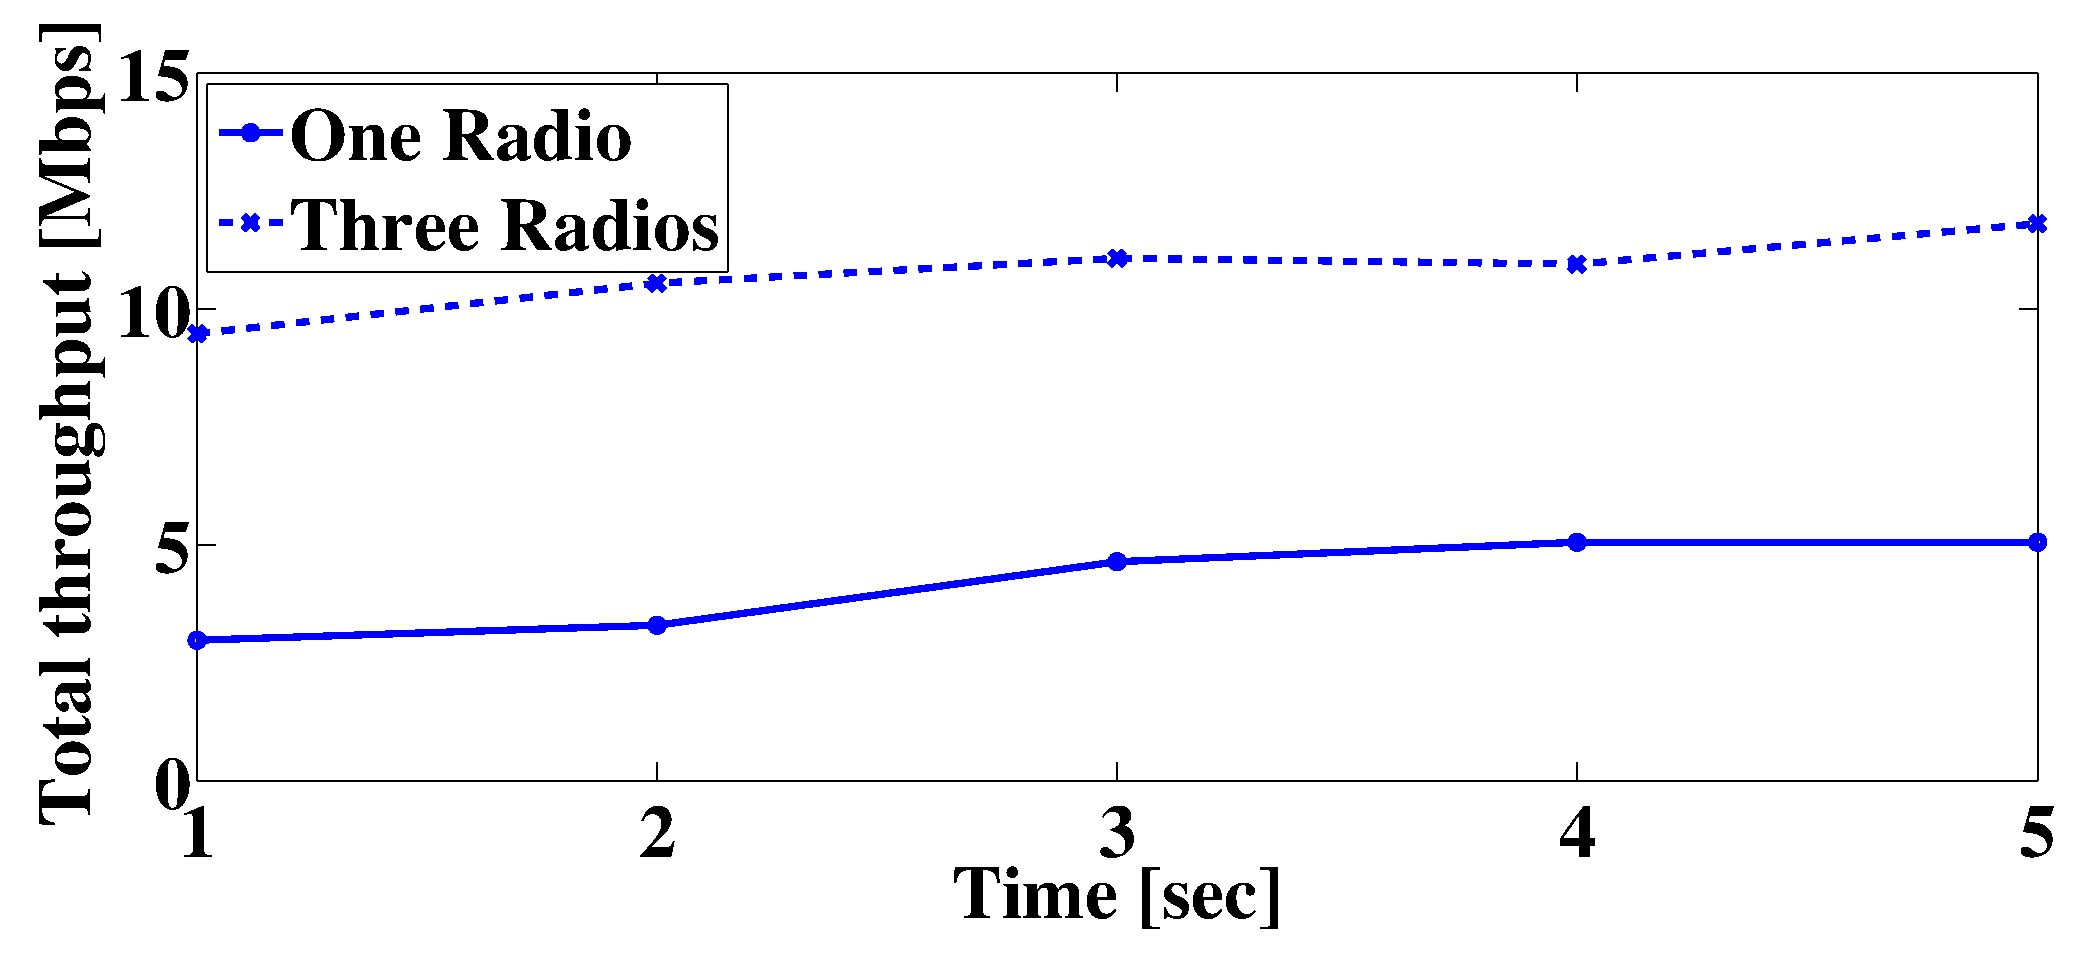
\includegraphics[width=0.5\textwidth]{3radio_vs_1radio.eps}}\\
        \caption{Comparison of total throughput for \algS in the grid
          scenario with $k=12$ and $d^*_i=50$Mbps. }
      \label{fig:radio13}
     \end{figure}

\paragraph{Fairness}
Figure~\ref{fig:fair} compares the sorted throughputs achieved for the
streams in \algA\ and \algS.  The experiment was made in the grid
arrangement, with $k=16$ streams and $d^*_i=50$ Mbps.

Although \algS\ has a higher total throughput, the $7$ with the
smallest throughputs have less throughput in \algS than in \algA.
This means that \algS favors short links, and is less fair than \algA.
\begin{figure}[h!]
      \centering
        \subfloat[]{\label{fig:small3}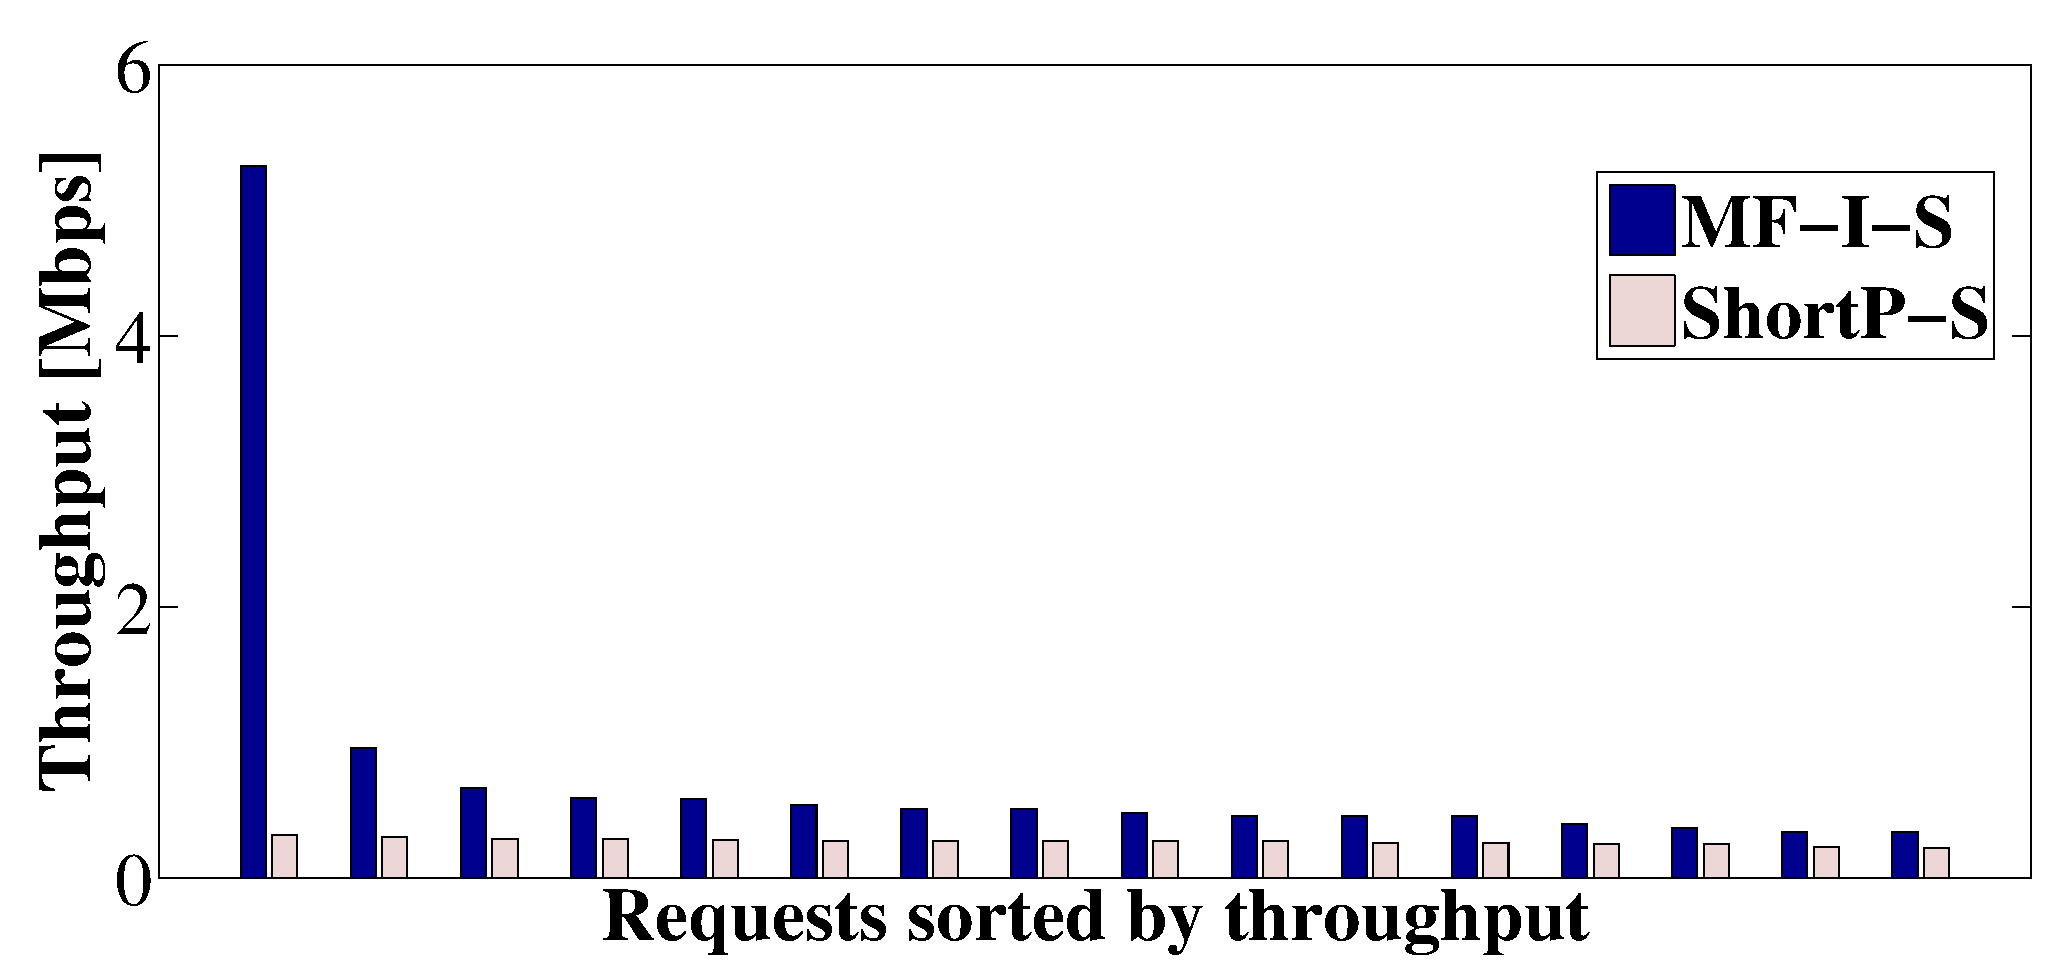
\includegraphics[width=0.5\textwidth]{fairness_compare.eps}}\\
        \caption{Streams in each benchmark are sorted by their
          throughput for the grid arrangement with $k=12$. }
      \label{fig:fair}
     \end{figure}

\paragraph{The Flow-Control algorithm}

Figure~\ref{fig:fcbig} depicts the effects of the Flow-Control
algorithm in the grid arrangement with $k=12$ and $d^*_i=50$Mbps.  In
Fig.~\ref{fig:fcsmall1}, the requested rates $R(e,s)$ are depicted. It
can be seen that only slight perturbations occur over time. This
justifies our simplified implementation that uses virtual flow-control messages.

In Fig.~\ref{fig:fcsmall2}, the queue lengths of the stream in three
different nodes are depicted.  The oscillation is due to the periodic
schedule. The queue length is controlled and stabilizes.

In Fig.~\ref{fig:fcsmall3}, the drop ratio is depicted for the worst
stream. The drop rate ranges from $0$ to $1.5$\%.

In Fig.~\ref{fig:fcsmall4}, the differences between the maximum and
minimum throughput for \algA\ and \algS\ are depicted for all streams
two seconds after the beginning of the experiment.
It is evident that \algA\ is more stable than \algS\ since the differences are smaller.

\begin{comment}
  \textbf{suggest other ways to implement the flow-control messages
    (incorporate in ACKs, send in the beginning of a time slot,
    reserve control slots).}
\end{comment}

\begin{figure}[h!]
      \centering
        \subfloat[Change in the requested packet rate by the flow-control over time]{\label{fig:fcsmall1}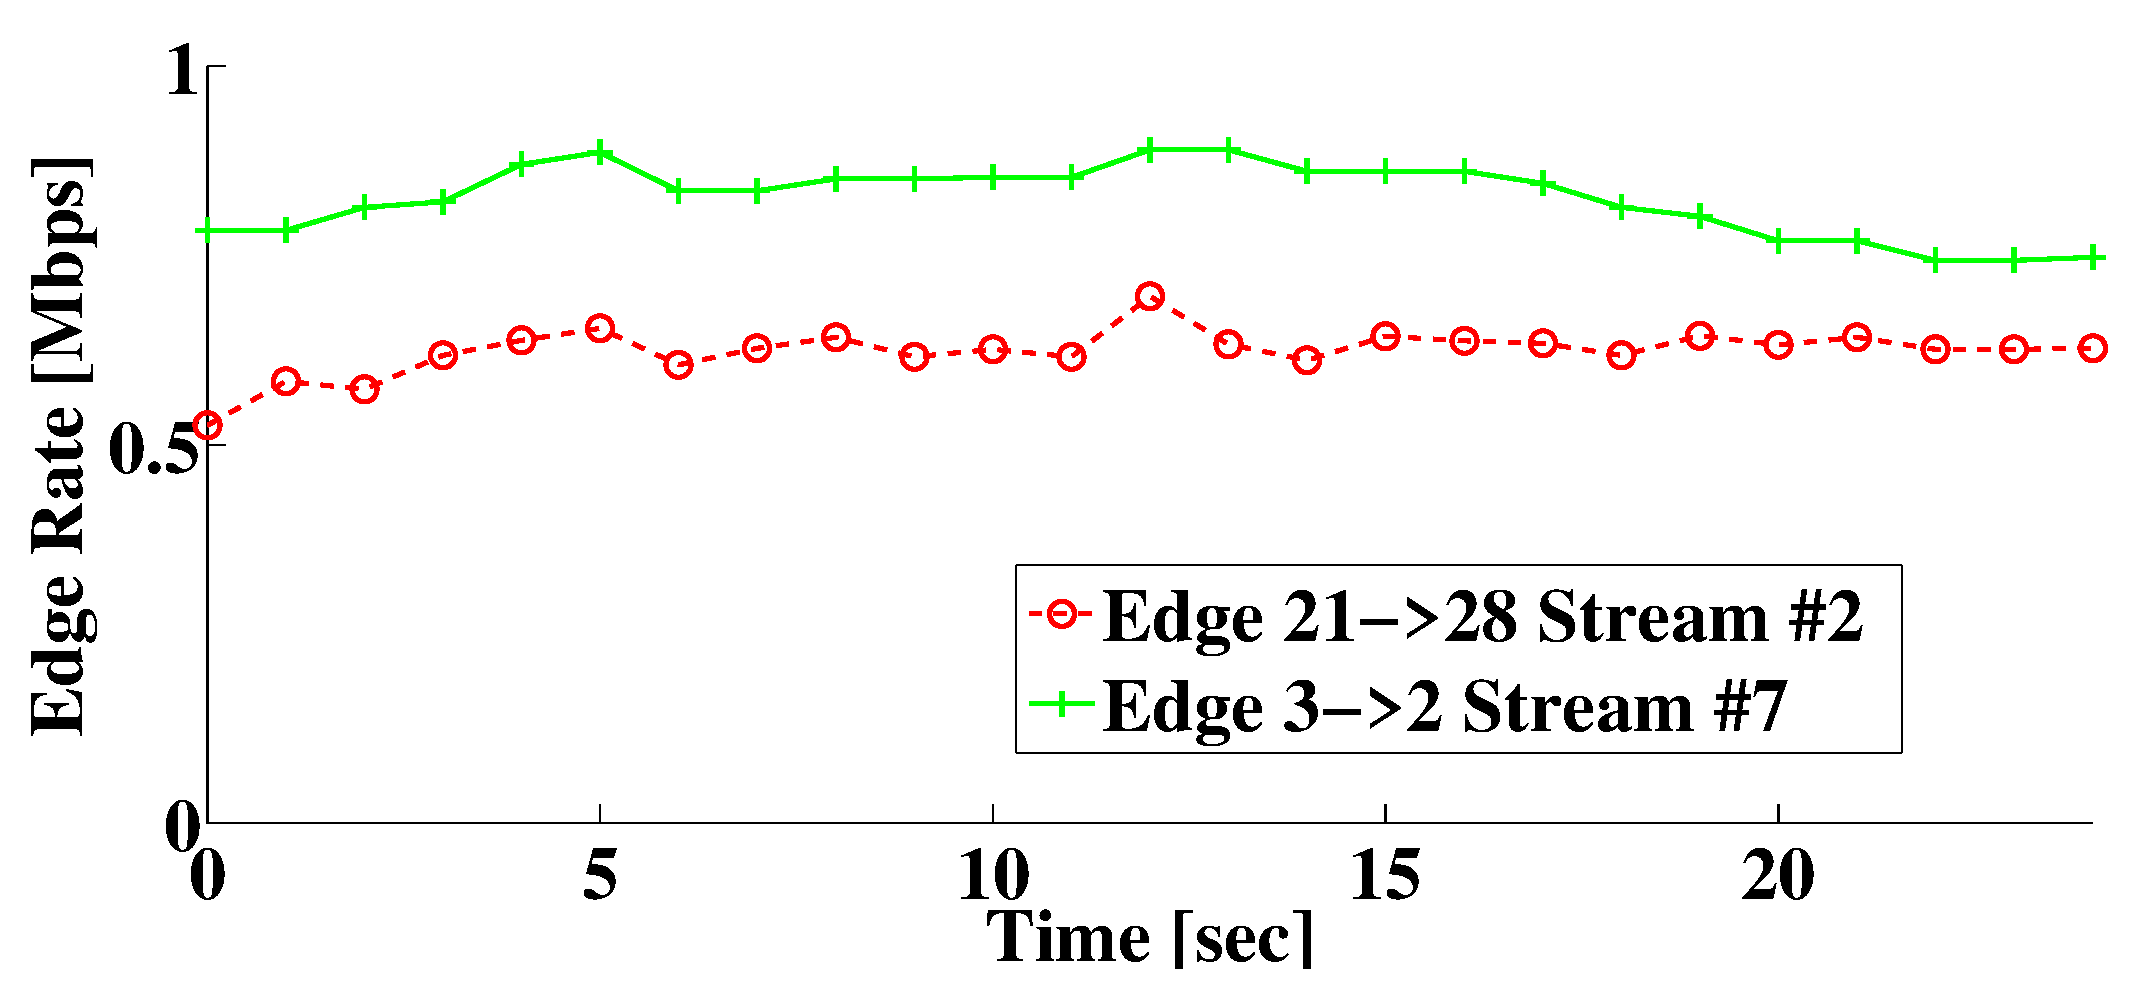
\includegraphics[width=0.5\textwidth]{fc_rate_long_grid_12r_new.eps}}\\
        \subfloat[Queue lengths of a stream in three different nodes]{\label{fig:fcsmall2}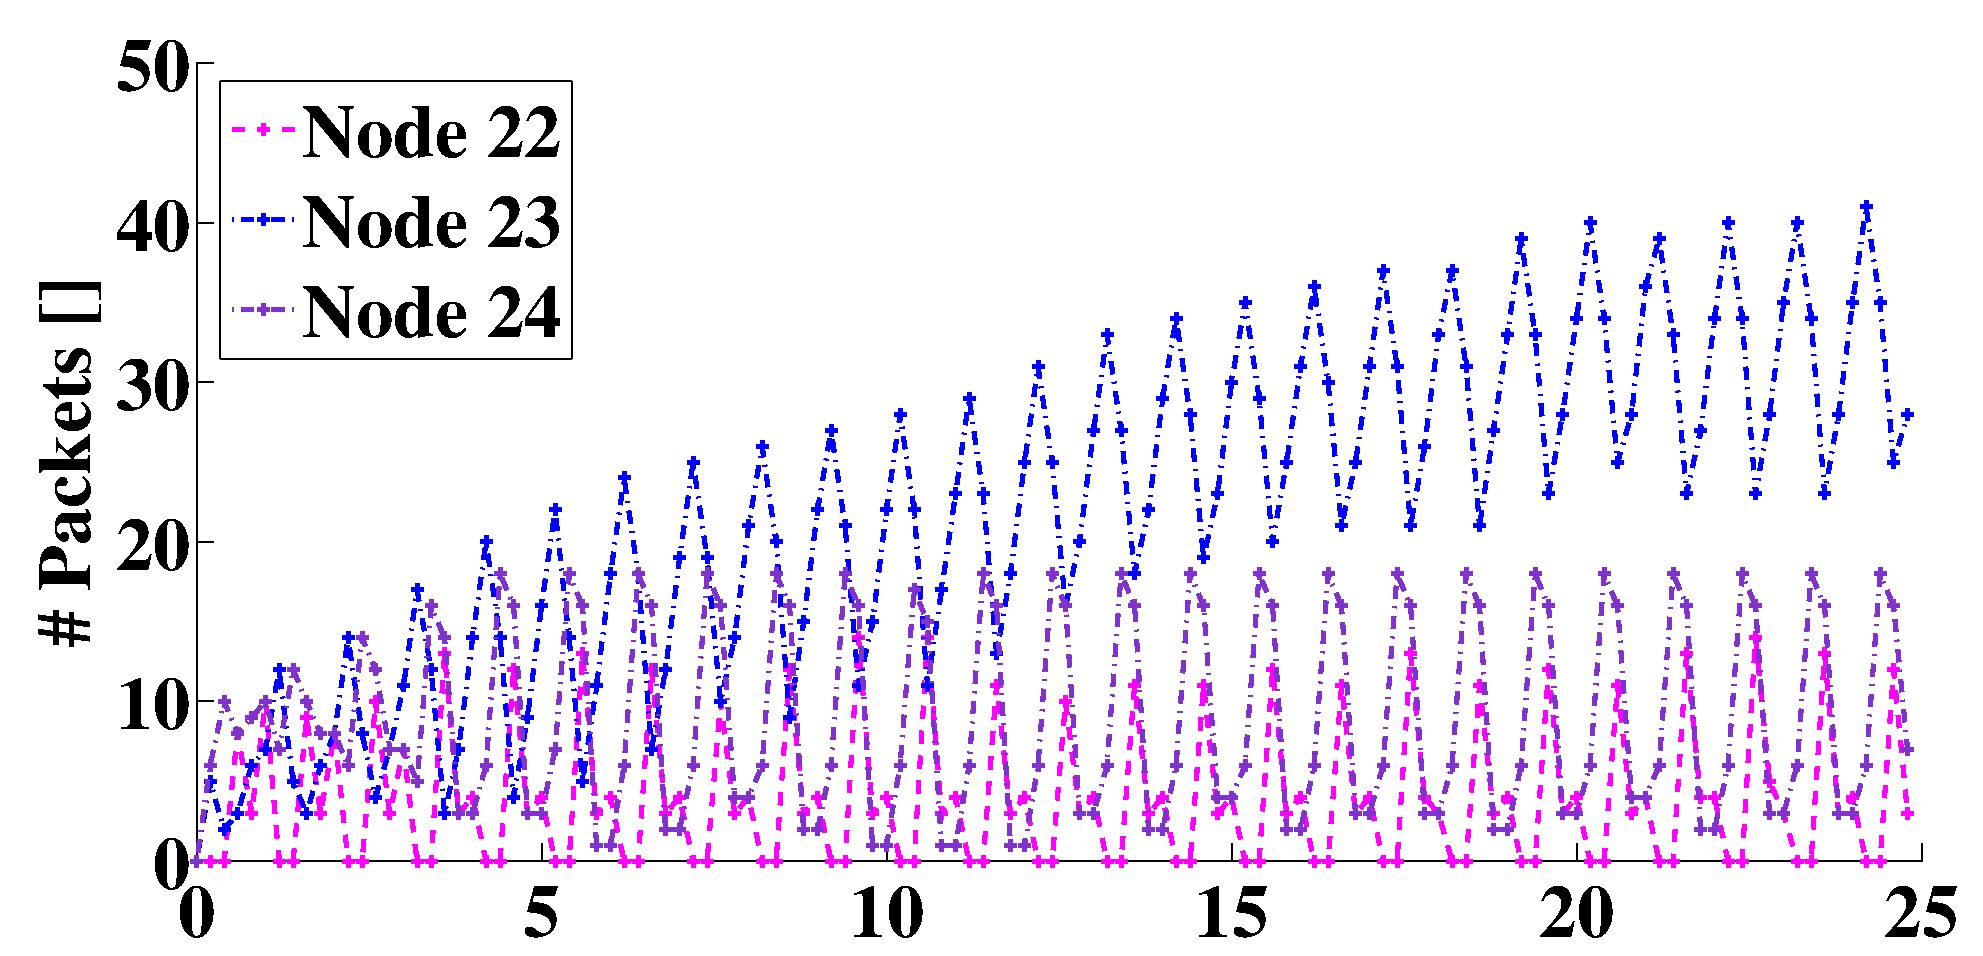
\includegraphics[width=0.5\textwidth]{q_len_max_multi_1_fig.eps}}\\
        \subfloat[Ratio of dropped packets to transmitted packets over time in worst stream]{\label{fig:fcsmall3}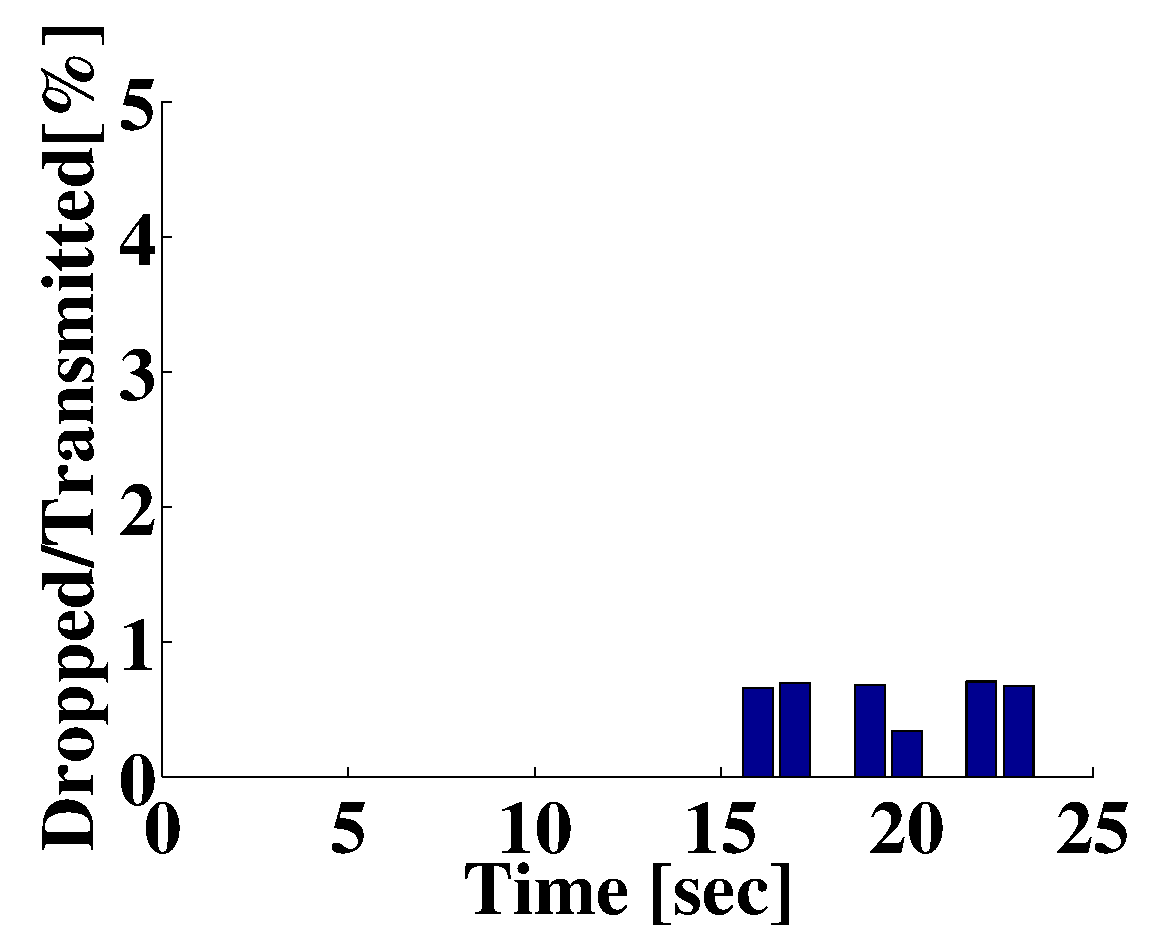
\includegraphics[width=0.5\textwidth]{max_drop_in_time_grid_12r.eps}}\\
        \subfloat[Comparison of stability of throughput between \algA\ and \algS ]{\label{fig:fcsmall4}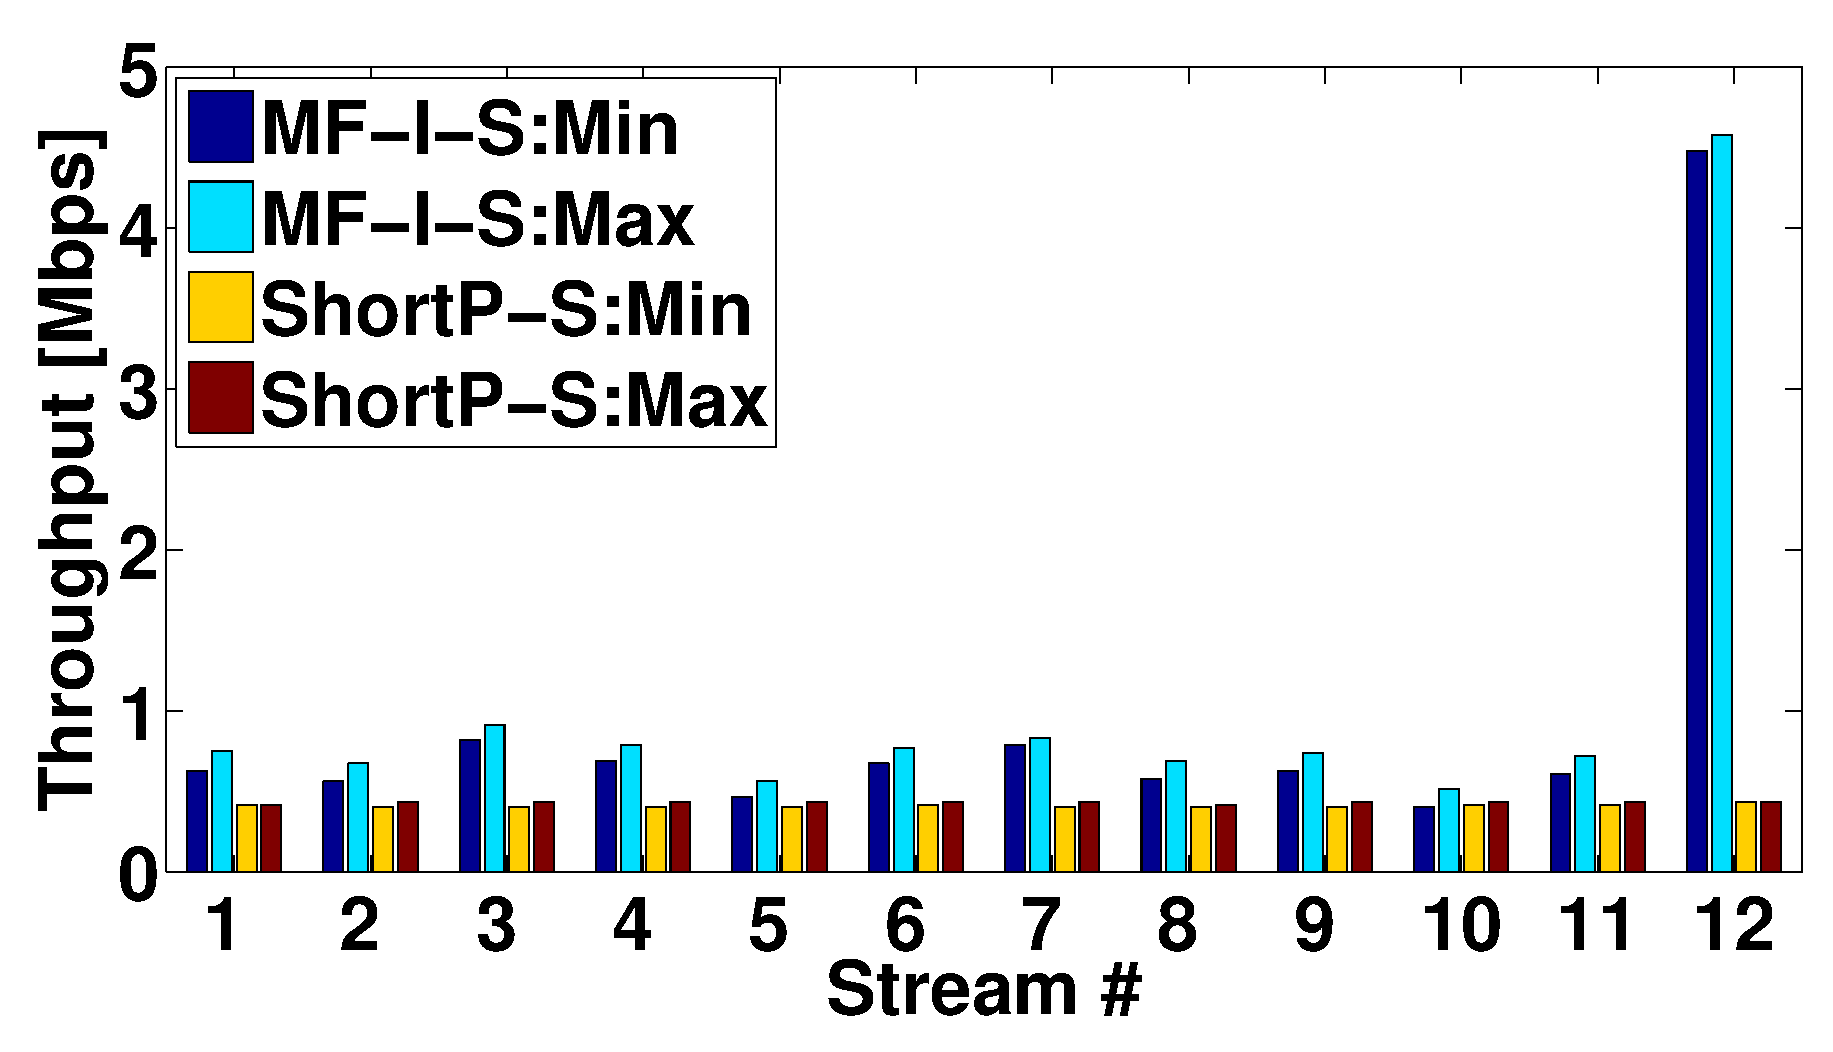
\includegraphics[width=0.5\textwidth]{tp_stability.eps}}\\
        \caption{Influence of the Flow-Control algorithm in  the grid arrangement with $k=12$
        }
    \label{fig:fcbig}
     \end{figure}


\paragraph{Comparison with greedy scheduler}
In Figure~\ref{fig:big3} we compare \algA\ with the greedy scheduler
and the path-peeling scheduler.  The throughput obtained with the
path-peeling scheduler is smaller, the end-to-end delay is
significantly improved.

\begin{figure}[h!]
  \centering
  \subfloat[Comparison of throughput]{\label{fig:small11}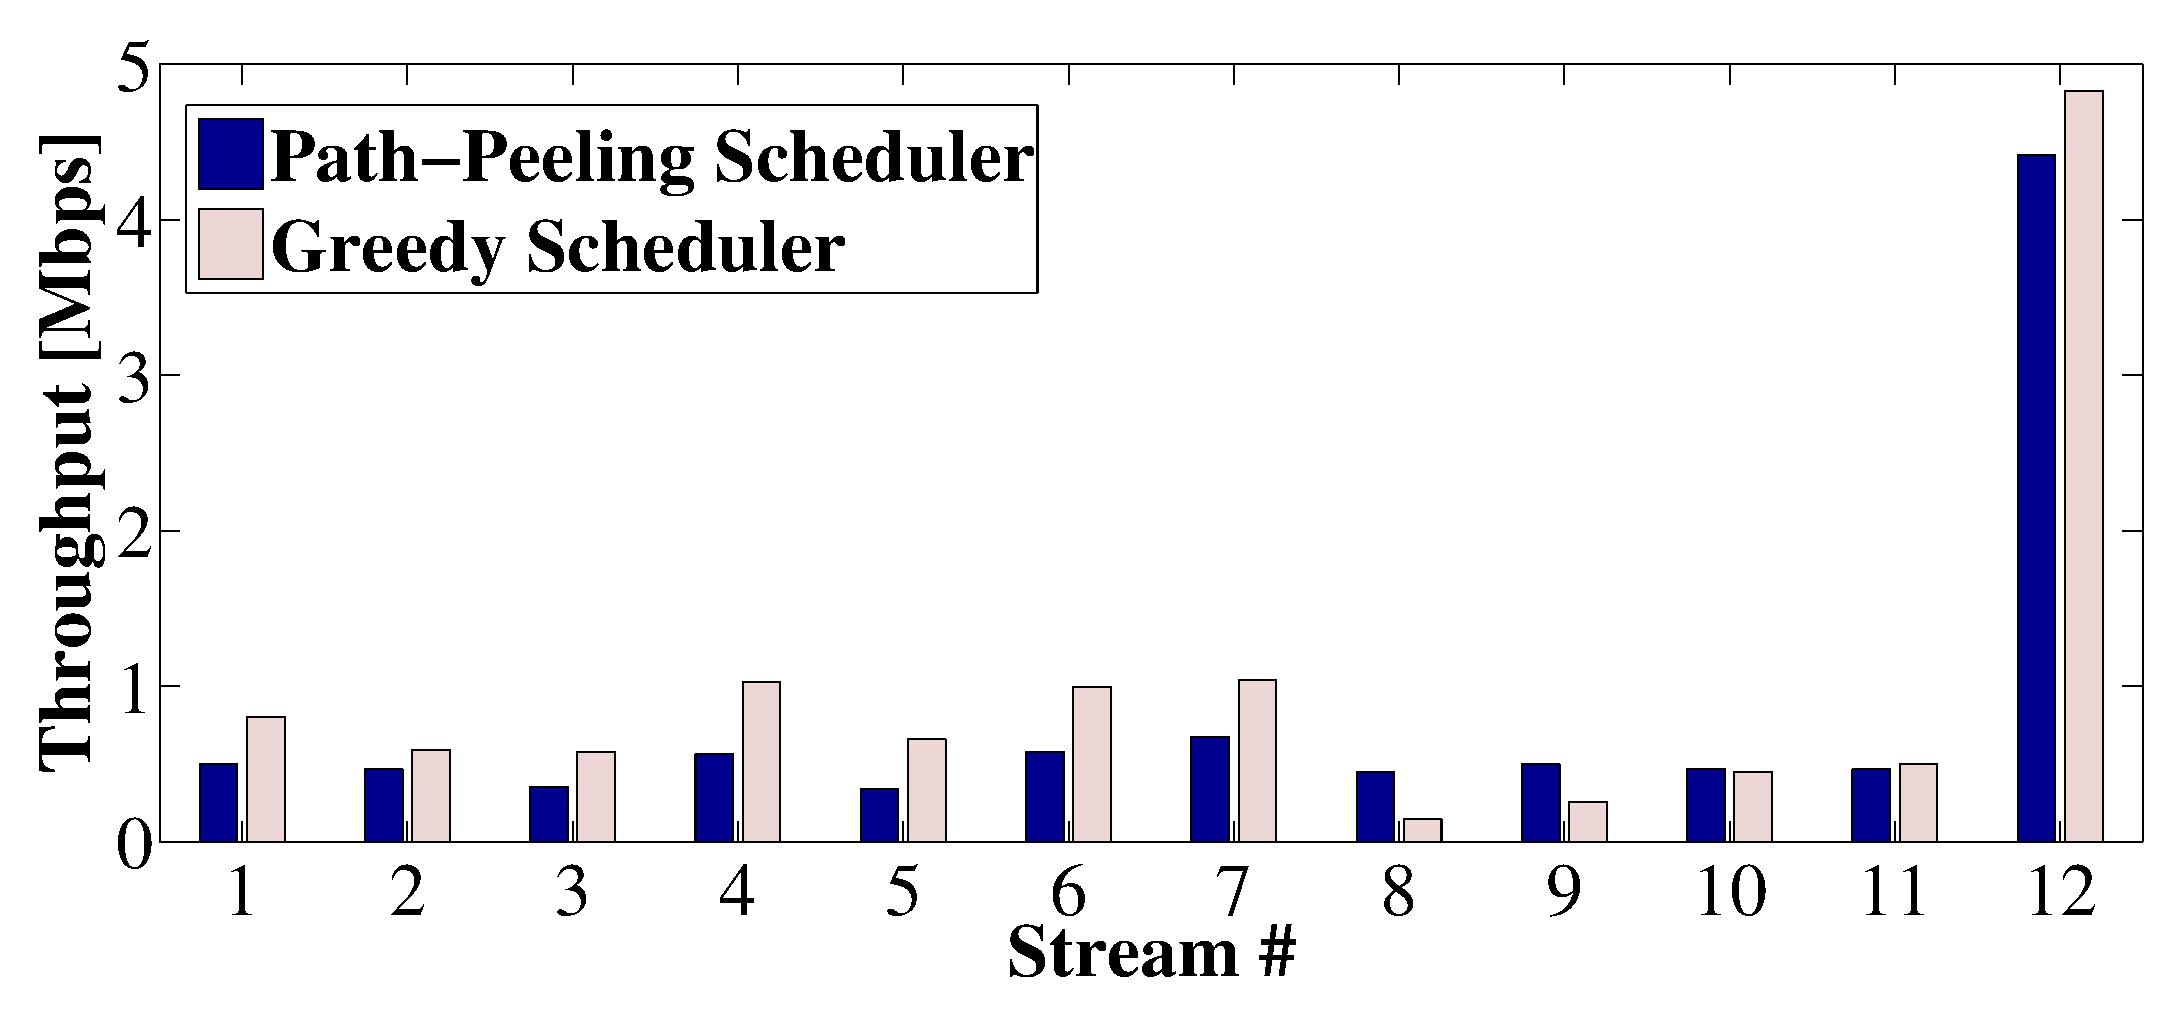
\includegraphics[width=0.5\textwidth]{tp_sched_comparison.eps}}\\
  \subfloat[Comparison of end-to-end delay]{\label{fig:small5}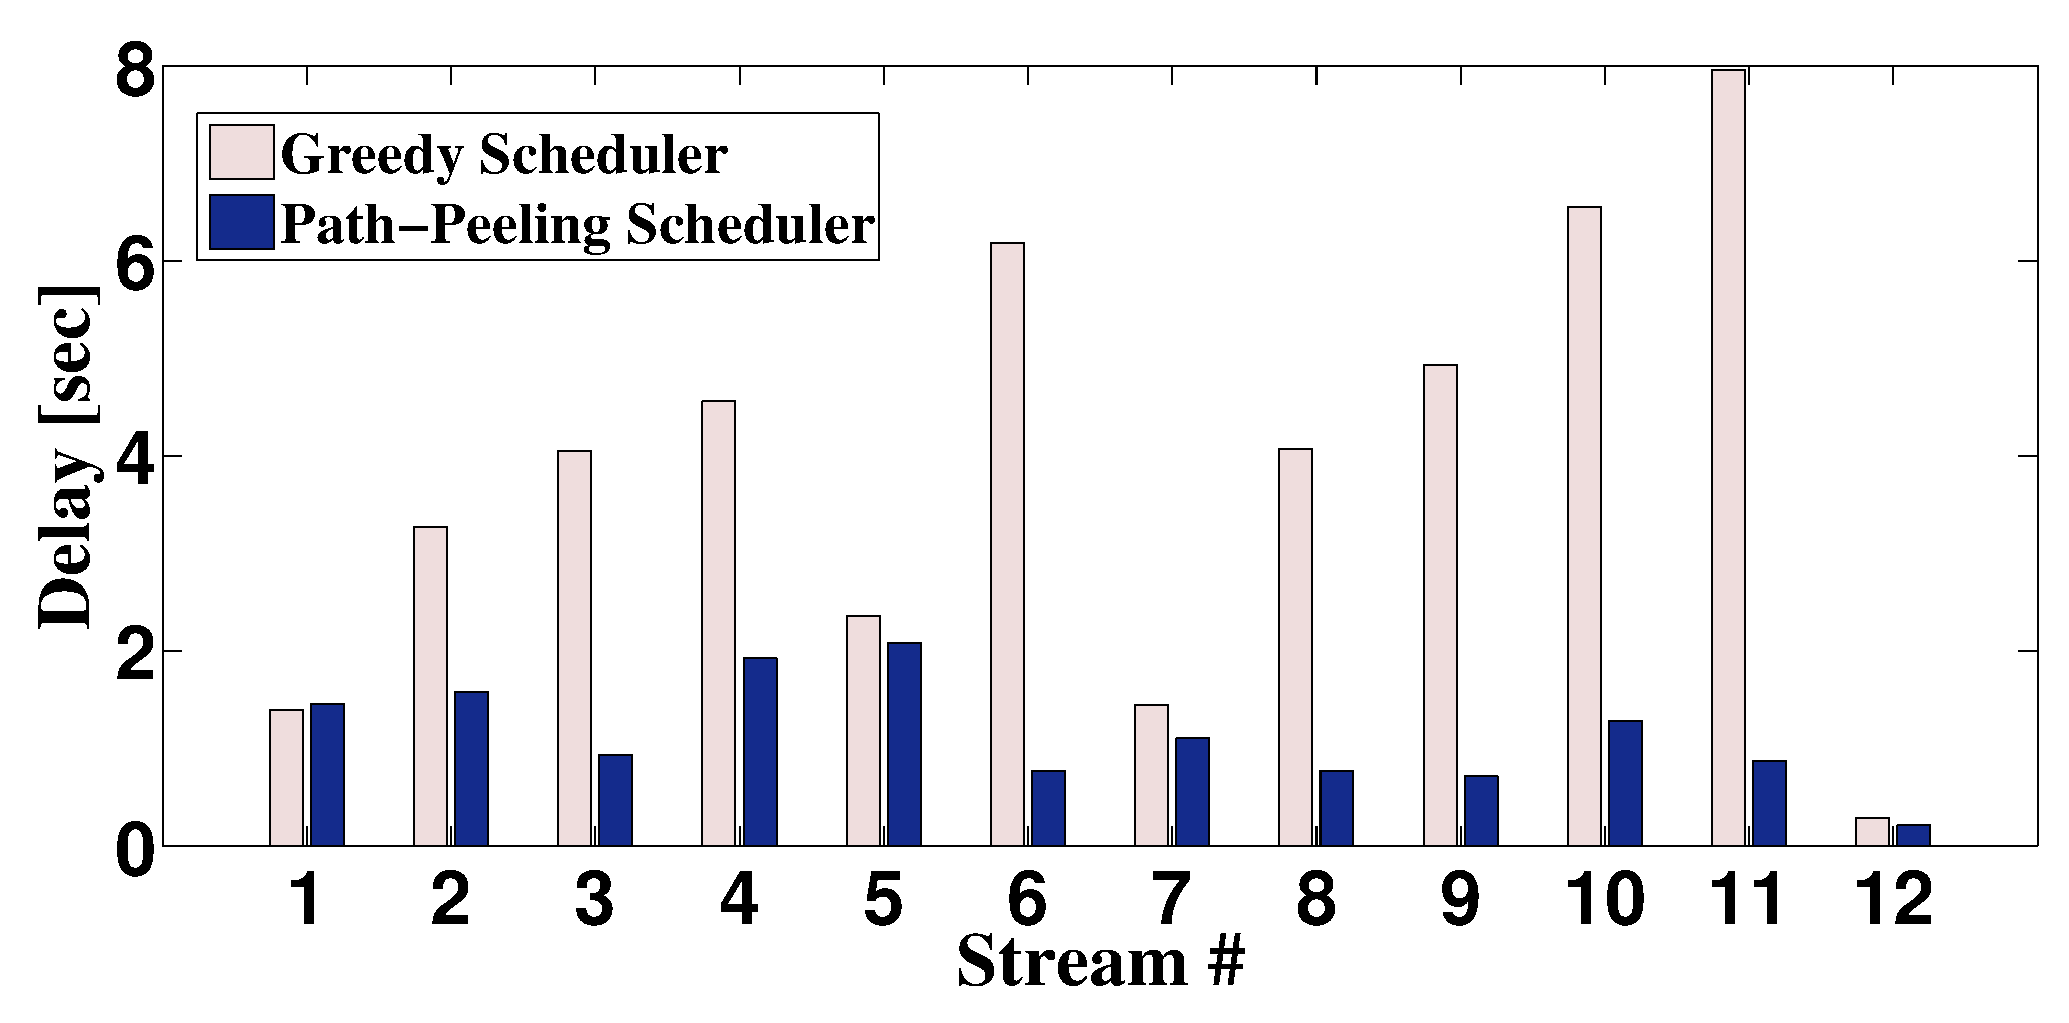
\includegraphics[width=0.5\textwidth]{max_delay_greedy_vs_smart.eps}}\\
  \subfloat[]{\label{fig:small9}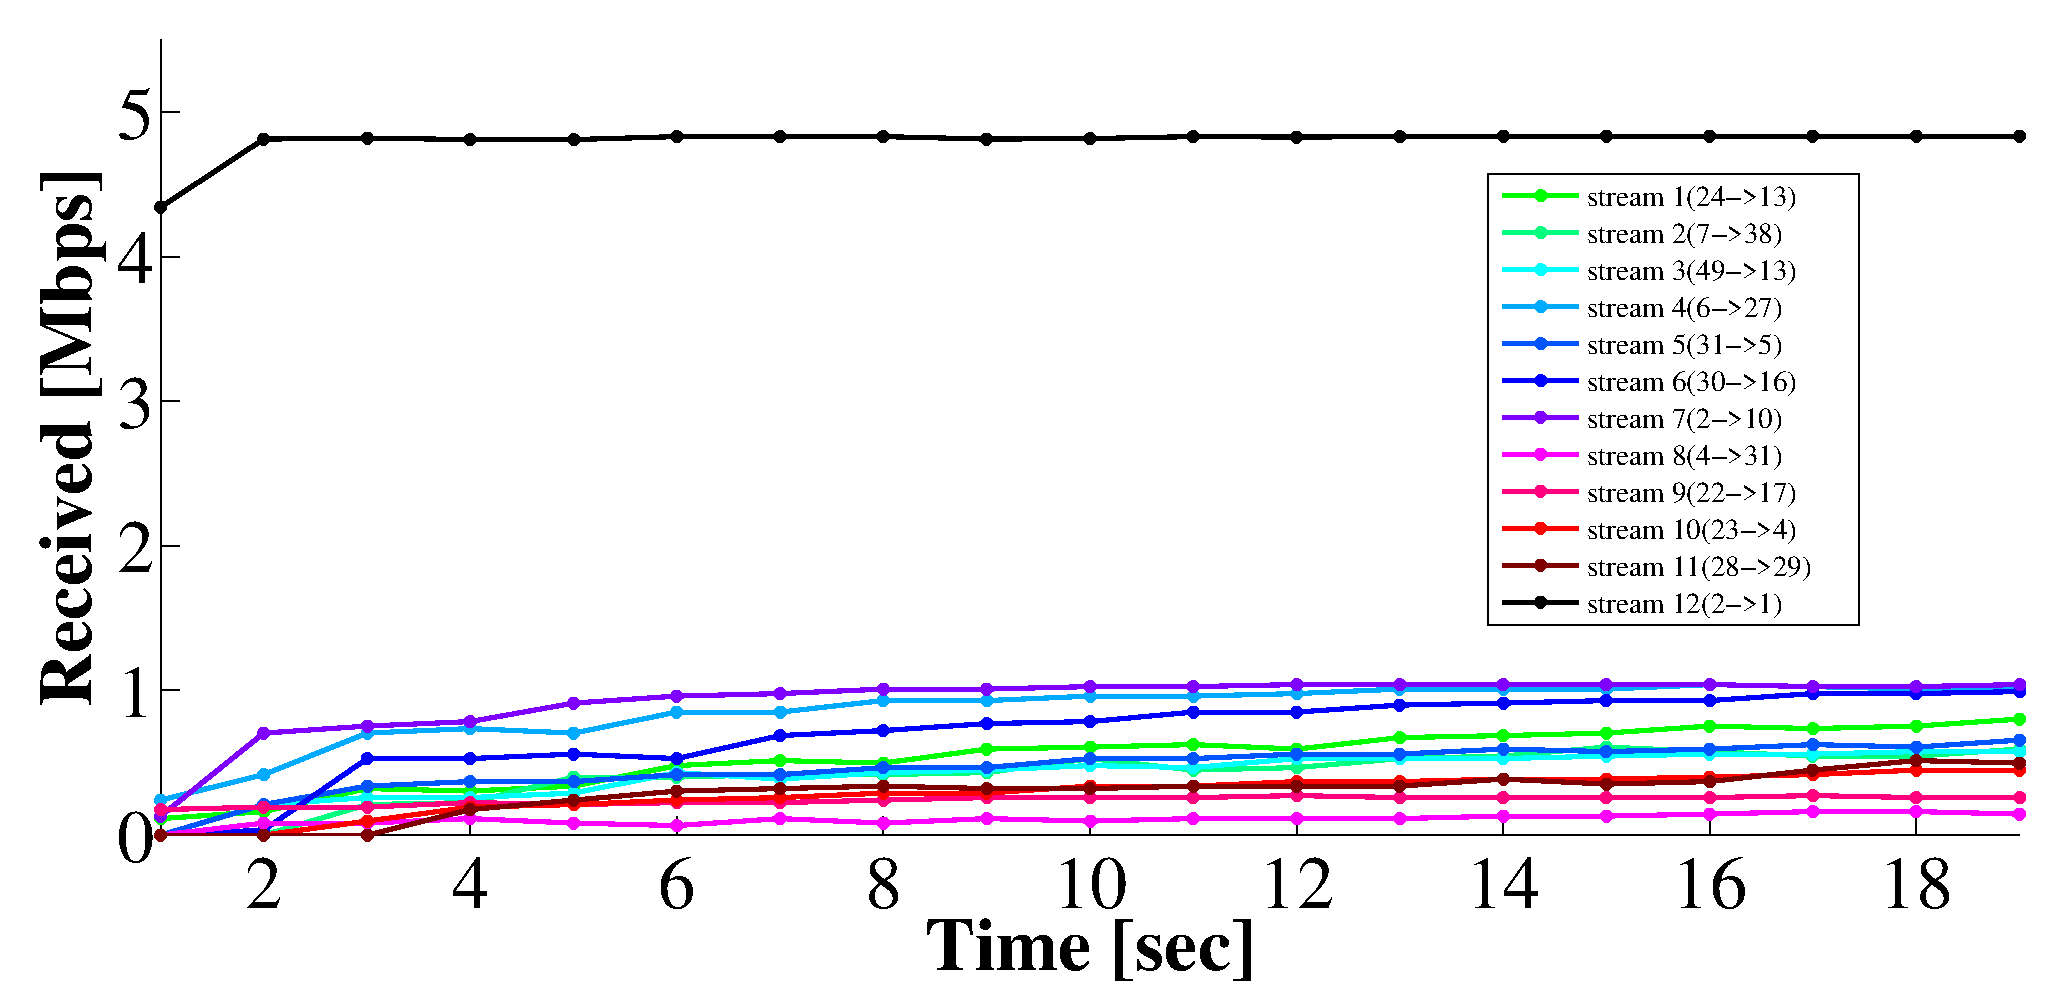
\includegraphics[width=0.5\textwidth]{throughput_greedy_sched_grid_12r.eps}}\\
  \subfloat[]{\label{fig:small10}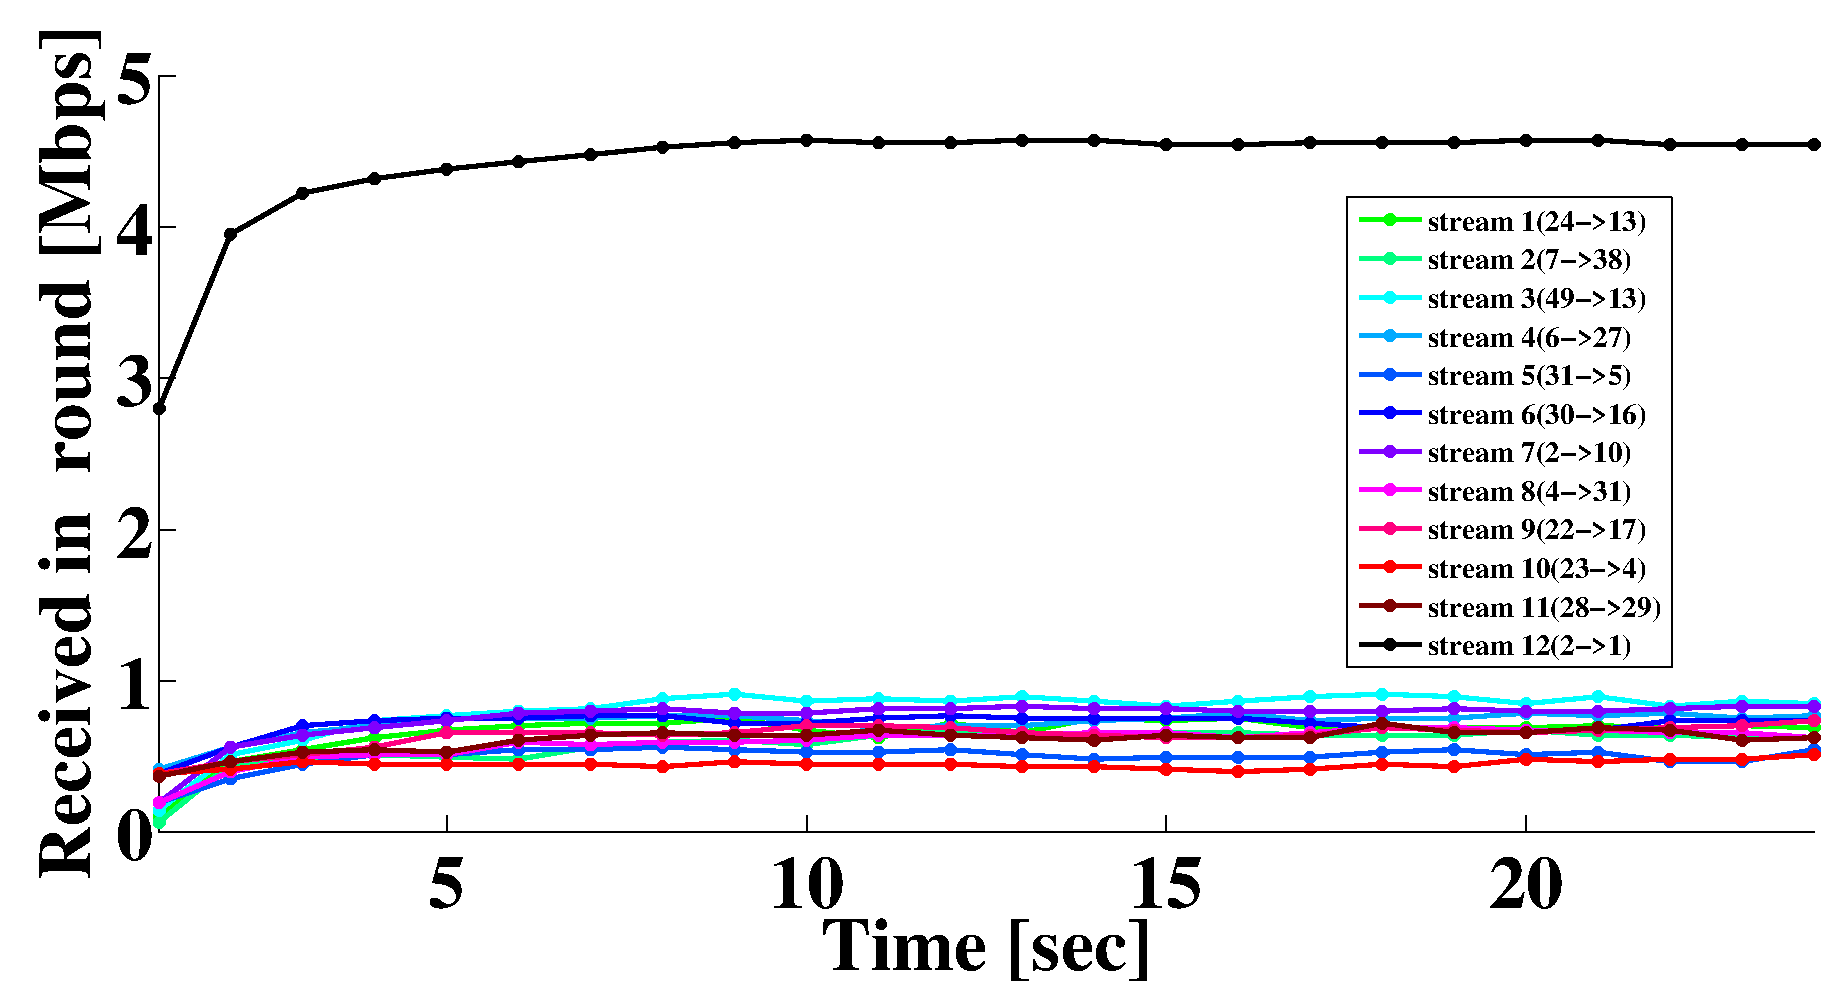
\includegraphics[width=0.5\textwidth]{throughput_smart_sched_grid_12r.eps}}\\
  \label{fig:big3}
\caption{Comparison of \algA\ with the greedy scheduler and the path-peeling scheduler}
     \end{figure}

\begin{table*}
\centering\scriptsize
\begin{tabular}{|| l || c | c | c | c | c|| c | c || c | c || c | c | c ||}
\hline
& \#radios  & \multicolumn{3}{|c|}{throughput}  & Delay & \multicolumn{4}{|c||}{delay based on hops} & hops & drops & \PER \\
\hline
& per node & min & sum & max & max & \multicolumn{2}{|c||}{max} & \multicolumn{2}{|c||}{min} & avr & max & avr \\
\hline
& & Mbps & Mbps & Mbps & sec & \#hops & sec & \#hops & sec & & \% & \% \\
\hline\hline
\algA & 1 & 0.512 & 12.08 & 4.544  & 2.25 & 14 & 2.25 & 1 & 0.2 & 7.17 & 0.7 & 1.85 \\
\algB & 3 & 0.064 &  8.9  & 1.568  &  \textbf{24}  &  9 &  23  & 1 & 1.35 & 4.5 & 24  & 1.09 \\
\algBS & 1 & 0.402  & 5.02 & 0.4342 & 1.5 & 9  & 1.32  & 1 & 0.95 & 4.5   & 0   & 0.15 \\
\algC & 3 & 0.064 & 4.32  & 1.2 & 3.9 & 14 & 2.6 & 1 & 1.2 & 7.17 & \textbf{95}   & 5.54 \\
\algD & 3 & 0 & 3.14  & 0.704  & 4.9 & 12 & 2.4  & 1 & 1.3  & 6.67  & \textbf{78}   & 6.63 \\
\algE & 1 & 0.1548  & 4.26  & 0.8  & \textbf{19}  & 12 & 15  & 1 & 3.7  & 6.67  &  0.5   & 0.87 \\
\hline
\end{tabular}
\caption{Comparison of the benchmarks for the grid scenario with $k=12$ requests and $d^*_i=10$Mbps for each stream. The experiment's duration is $25$ seconds. }
\label{table_grid}\label{tbl:grid}
%\end{table*}


%\begin{table*}
\centering\scriptsize
\begin{tabular}{|| l || c | c | c | c | c|| c | c || c | c || c | c | c ||}
\hline
& \#radios  & \multicolumn{3}{|c|}{throughput}  & Delay & \multicolumn{4}{|c||}{delay based on hops} & hops & drops & \PER \\
\hline
& per node & min & sum & max & max & \multicolumn{2}{|c||}{max} & \multicolumn{2}{|c||}{min} & avr & max & avr \\
\hline
& & Mbps & Mbps & Mbps & sec & \#hops & sec & \#hops & sec & & \% & \% \\
\hline\hline
\algA & 1 &  2.37 & 32.1  & 2.97 & 1.23 & 2 & 1.23 & 2 & 0.68 & 2 & 0   & 0 \\
\algB & 3 & 4.82 & 56.2 & 4.88  & 2.5  & 2  & 2.5  & 2 & 1  & 2     & 34   & 0 \\
\algBS & 1 & 1.98 & 30.4 & 2.78  & \textbf{5.35}  & 2  & 4.1  & 2 & 0.35  & 2     & 0   & 0 \\
\algC & 3 & 1.35  & 18.4 & 1.75  & 1.5 & 2 & 1.5  & 2 & 1 & 2 & \textbf{36}  & 3 \\
\algD & 3 &  1.3 & 17.7 & 1.7 & 1.7 & 2 & 1.7  & 2 & 1 & 2 & \textbf{14}  & 2.48 \\
\algE & 1 &  0.85 & 15.42 & 1.75 & 2.64  & 2 & 2.64 & 2 & 4  & 2 & 0.65 & 0 \\
\hline
\end{tabular}
\caption{Comparison of the benchmarks for the circle scenario with $k=12$ requests and $d^*_i=10$Mbps for each stream. The experiment's duration is $25$ seconds. }
\label{table_circle}\label{tbl:circle}
\end{table*}



%%%%%% Scenarios and benchmarks
\begin{figure}%[h!]
      \centering
        \subfloat{\label{fig:small18}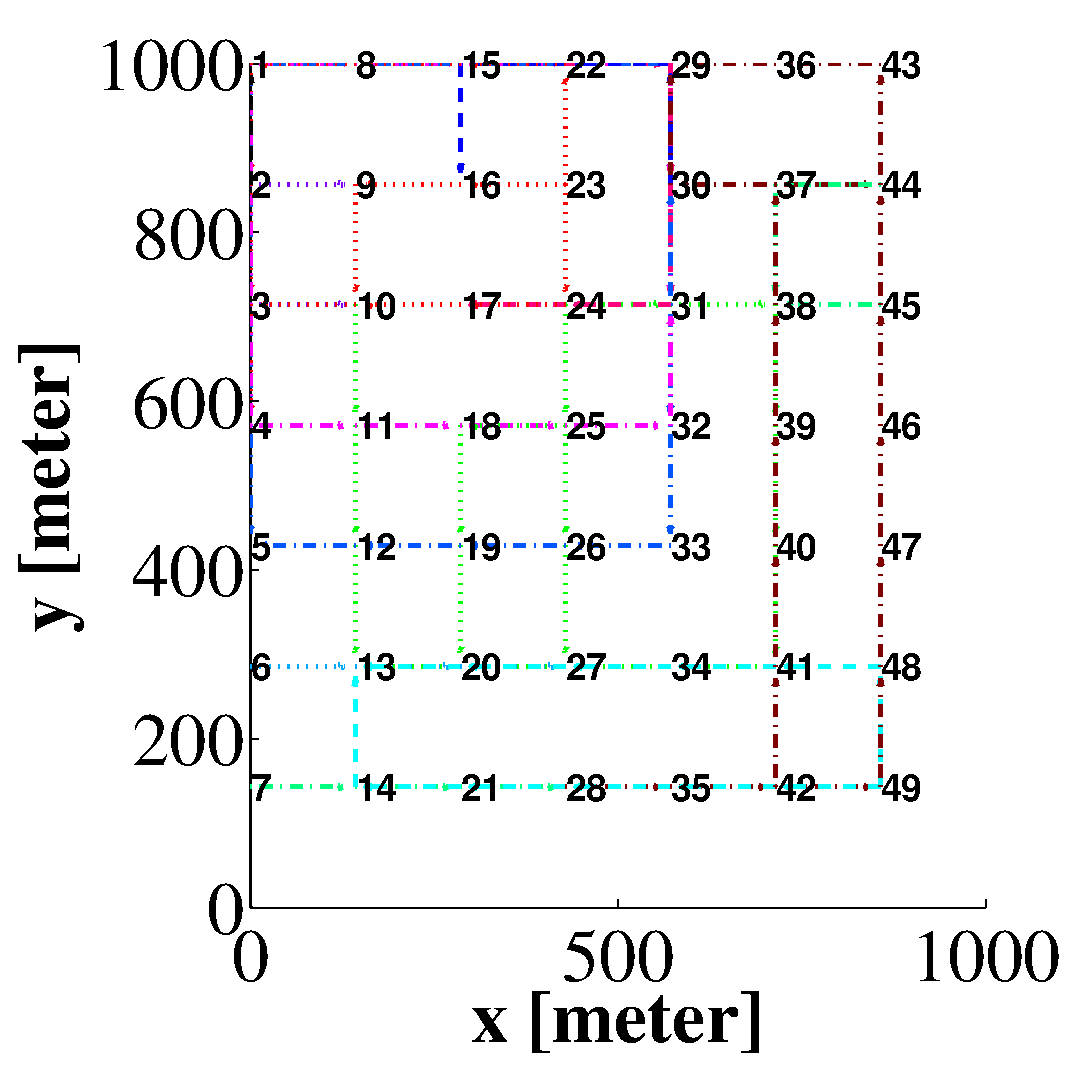
\includegraphics[width=0.4\textwidth, height = 0.4\textheight]{scenario_main_grid_12r.eps}}
       \caption{The grid scenario with $49$ nodes}
      \label{fig:big6}\label{fig:scenario grid}
     \end{figure}

\begin{figure}%[h!]
      \centering
        \subfloat{\label{fig:small13}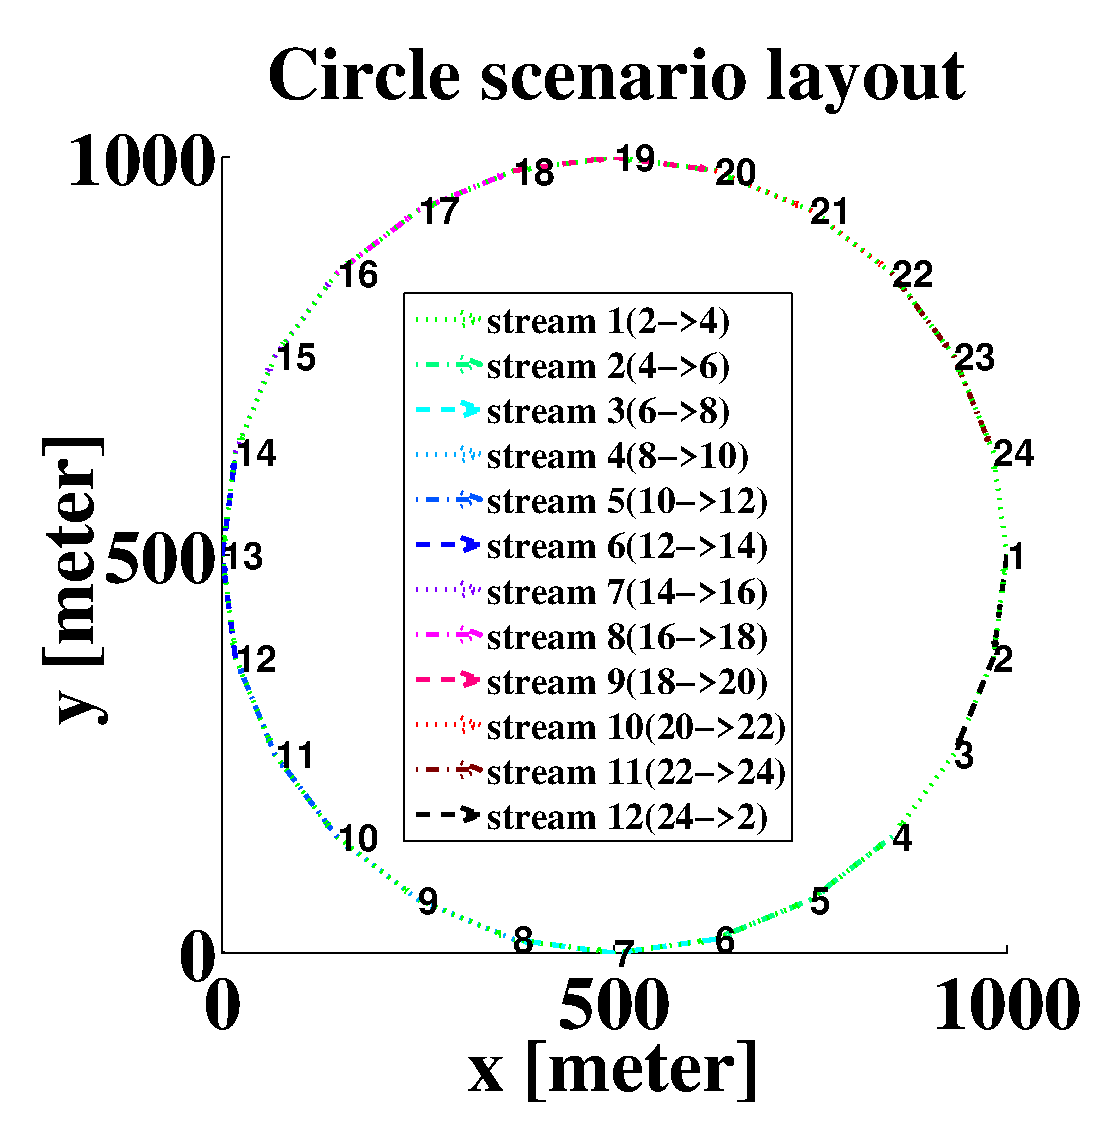
\includegraphics[width=0.5\textwidth, height = 0.5\textheight]{scenario_main_circle_12d.eps}}
        \caption{The circle scenario with $24$ nodes}
      \label{fig:big5}\label{fig:scenario circle}
     \end{figure}

\section{Conclusions}
In terms of the stream with the minimum throughput, \algA\ outperforms
the \algS\ algorithm with a single WNIC. In the grid, \algA\ even
outperforms \algS\ with $3$ WNICS per node.  We attribute this to the
routing that may use multiple paths per stream.

In terms of end-to-end delay, \algA\ outperforms all the benchmarks
even when it uses paths that are much longer.

The average drop rate for \algA\ is below $0.2$\%. This makes the algorithm
feasible for reliable communication of real-time video streams.

We summarize our conclusions by noting that the performance of \algA\
is stable and predictable, and competes well with nodes equipped with
$3$ radios in the \algS\ benchmark.

\section{Discussion}
We propose a centralized algorithm for computing a routing,
scheduling, and frequency assignment for real-time video streams in
static ad hoc wireless networks.  The algorithm consists of two parts:
a linear program and a scheduler.  In addition, each node locally runs
a flow-control algorithm to control the queues and stabilize data-rate
along the links.  Although the algorithm is centralized, it can be
executed by multiple nodes in the network provided that they hold full
information of the network (i.e., locations, requests).  The output of
the algorithm consists two tables that easily be broadcast to all the
nodes.

We implemented the algorithm and experimented using a setting that
uses the physical model to verify the validity of the algorithm.  Our
experiments show that the algorithm performs well in two congested
scenarios.  

Future work should address methods for approximate distributed
algorithms for solving the linear program and for scheduling. In
addition, it is interesting to study the performance of the algorithm
when users are mobile.  It may be the case that performance does not
degrade quickly, so that new tables can be recalculated continuously.


%
\ifnum\conff=0
  \subsection*{Acknowledgments}
  We thank Nissim Halabi for useful discussions.
\fi
%

%\nocite{*}
\bibliographystyle{alpha}
\bibliography{wireless}
\end{document}
